\section{Design}

\subsection{Constraints and Goals} \label{Sec:ConstraintsandGoals}

The following constraints were identified prior to design:

\begin{itemize}
	\item Must mount to the existing filament holder location with no
	permanent modification to the printer frame.
	\item Must accommodate filament [diameter, 1.75\,mm]
	without excessive clearance that could cause buckling.
	\item Bend radius must be sufficient to prevent filament binding or
	fatigue cracking during continuous use.
	\item Should print without support material where possible to
	minimise post-processing.
	\item Must be set high enough so the filament line cannot collide with larger prints. 
	\item Must be able to withstand the partial weight of the dryer, approximately 1\,kg (Sometimes filament gets tangled inside the dryer and pulls the dryer over.).  
	\item Must be able to resist heat that is generated from the printing of parts 
	on the Ender 3. 
	\item Must allow  for a minimum radius of 35\,mm. This number was taken from the measurement of a spool. 
	 
\end{itemize}

\subsection{Design Concepts}
There are two major considerations for the filament design that need to be considered.
 The interface with the \Printername, and how the filament is to be guided. These considerations
  will be evaluated independently then combined together as the final design. 
  

\subsubsection{Frame Mounting Design}
%---------Twist lock-------------------------
%--------------------------------------------
\paragraph{Twist Lock} One concept for the attachment of the Filament Guide would be to reuse the original handle that holds up the filament spool. This could be a simple and proven design that has been shown to work. The original attachment as well as the printed concept can be seen in Fig.\ref{fig:OrignalDesignConcept}. 


\begin{figure}[tbh!]
	\centering
	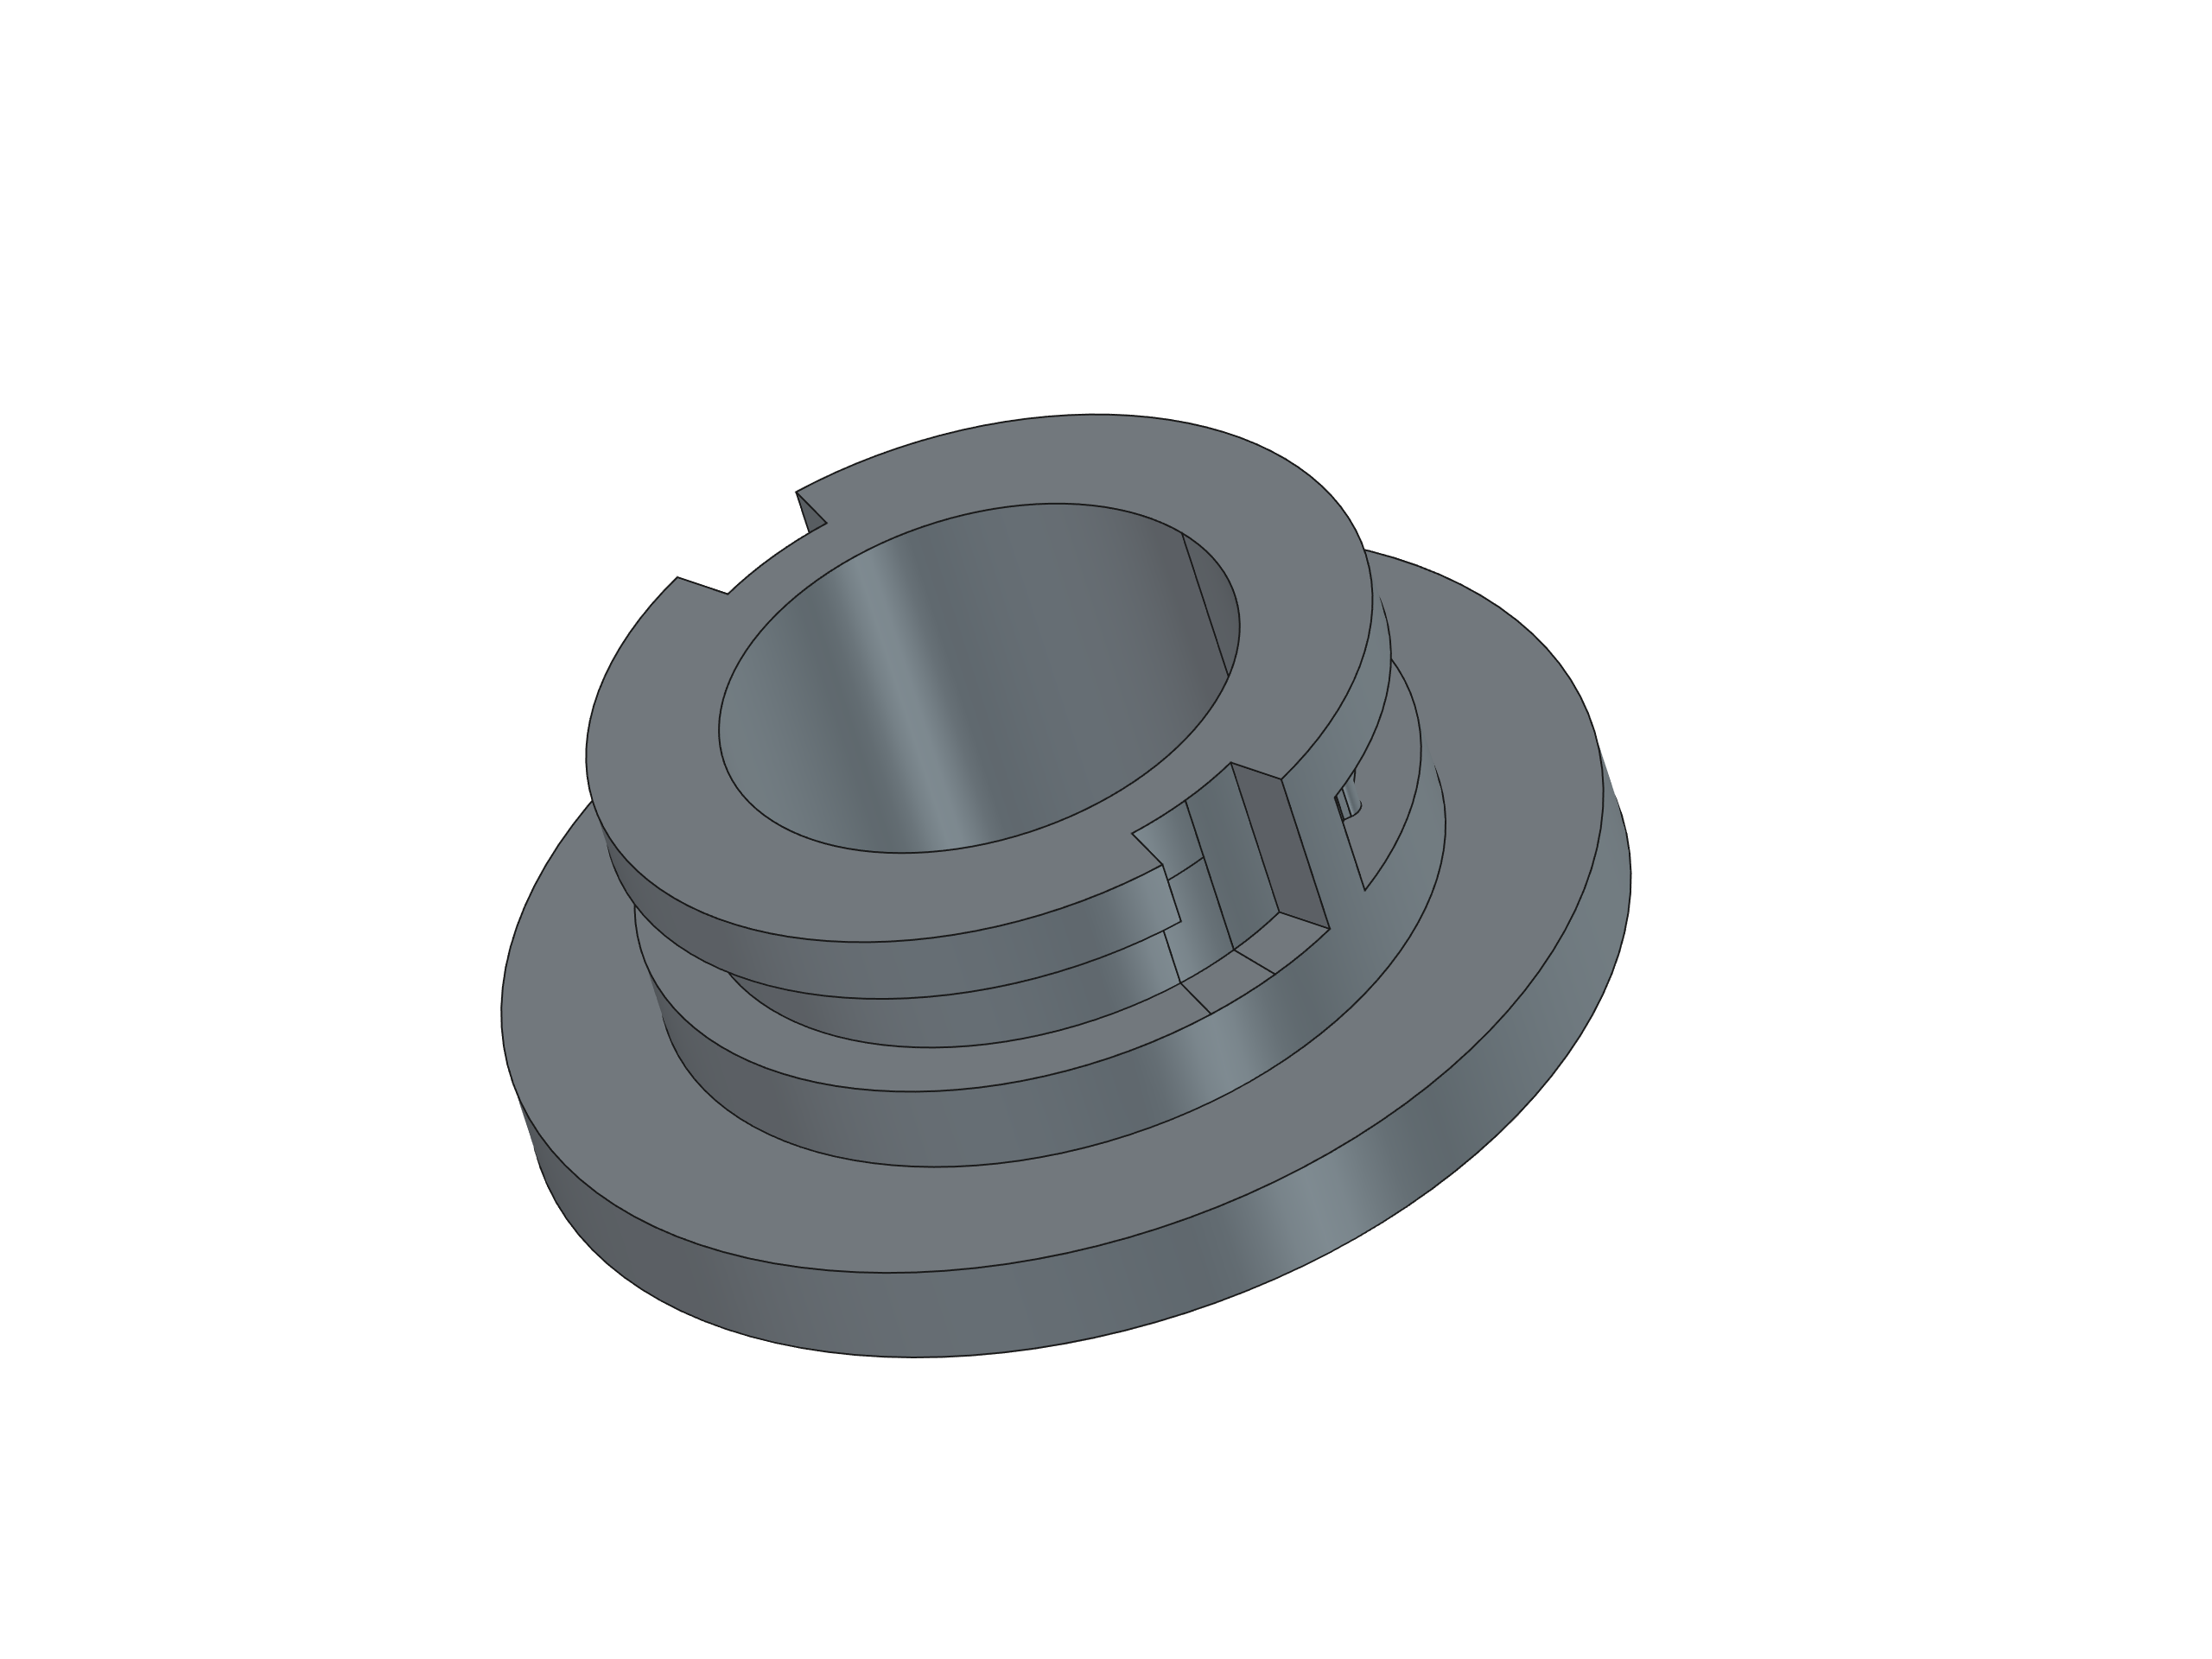
\includegraphics[width={\dimexpr\textwidth/2 - 6pt - 1pt\relax}]{./Images/OriginalMountRemade.png}
	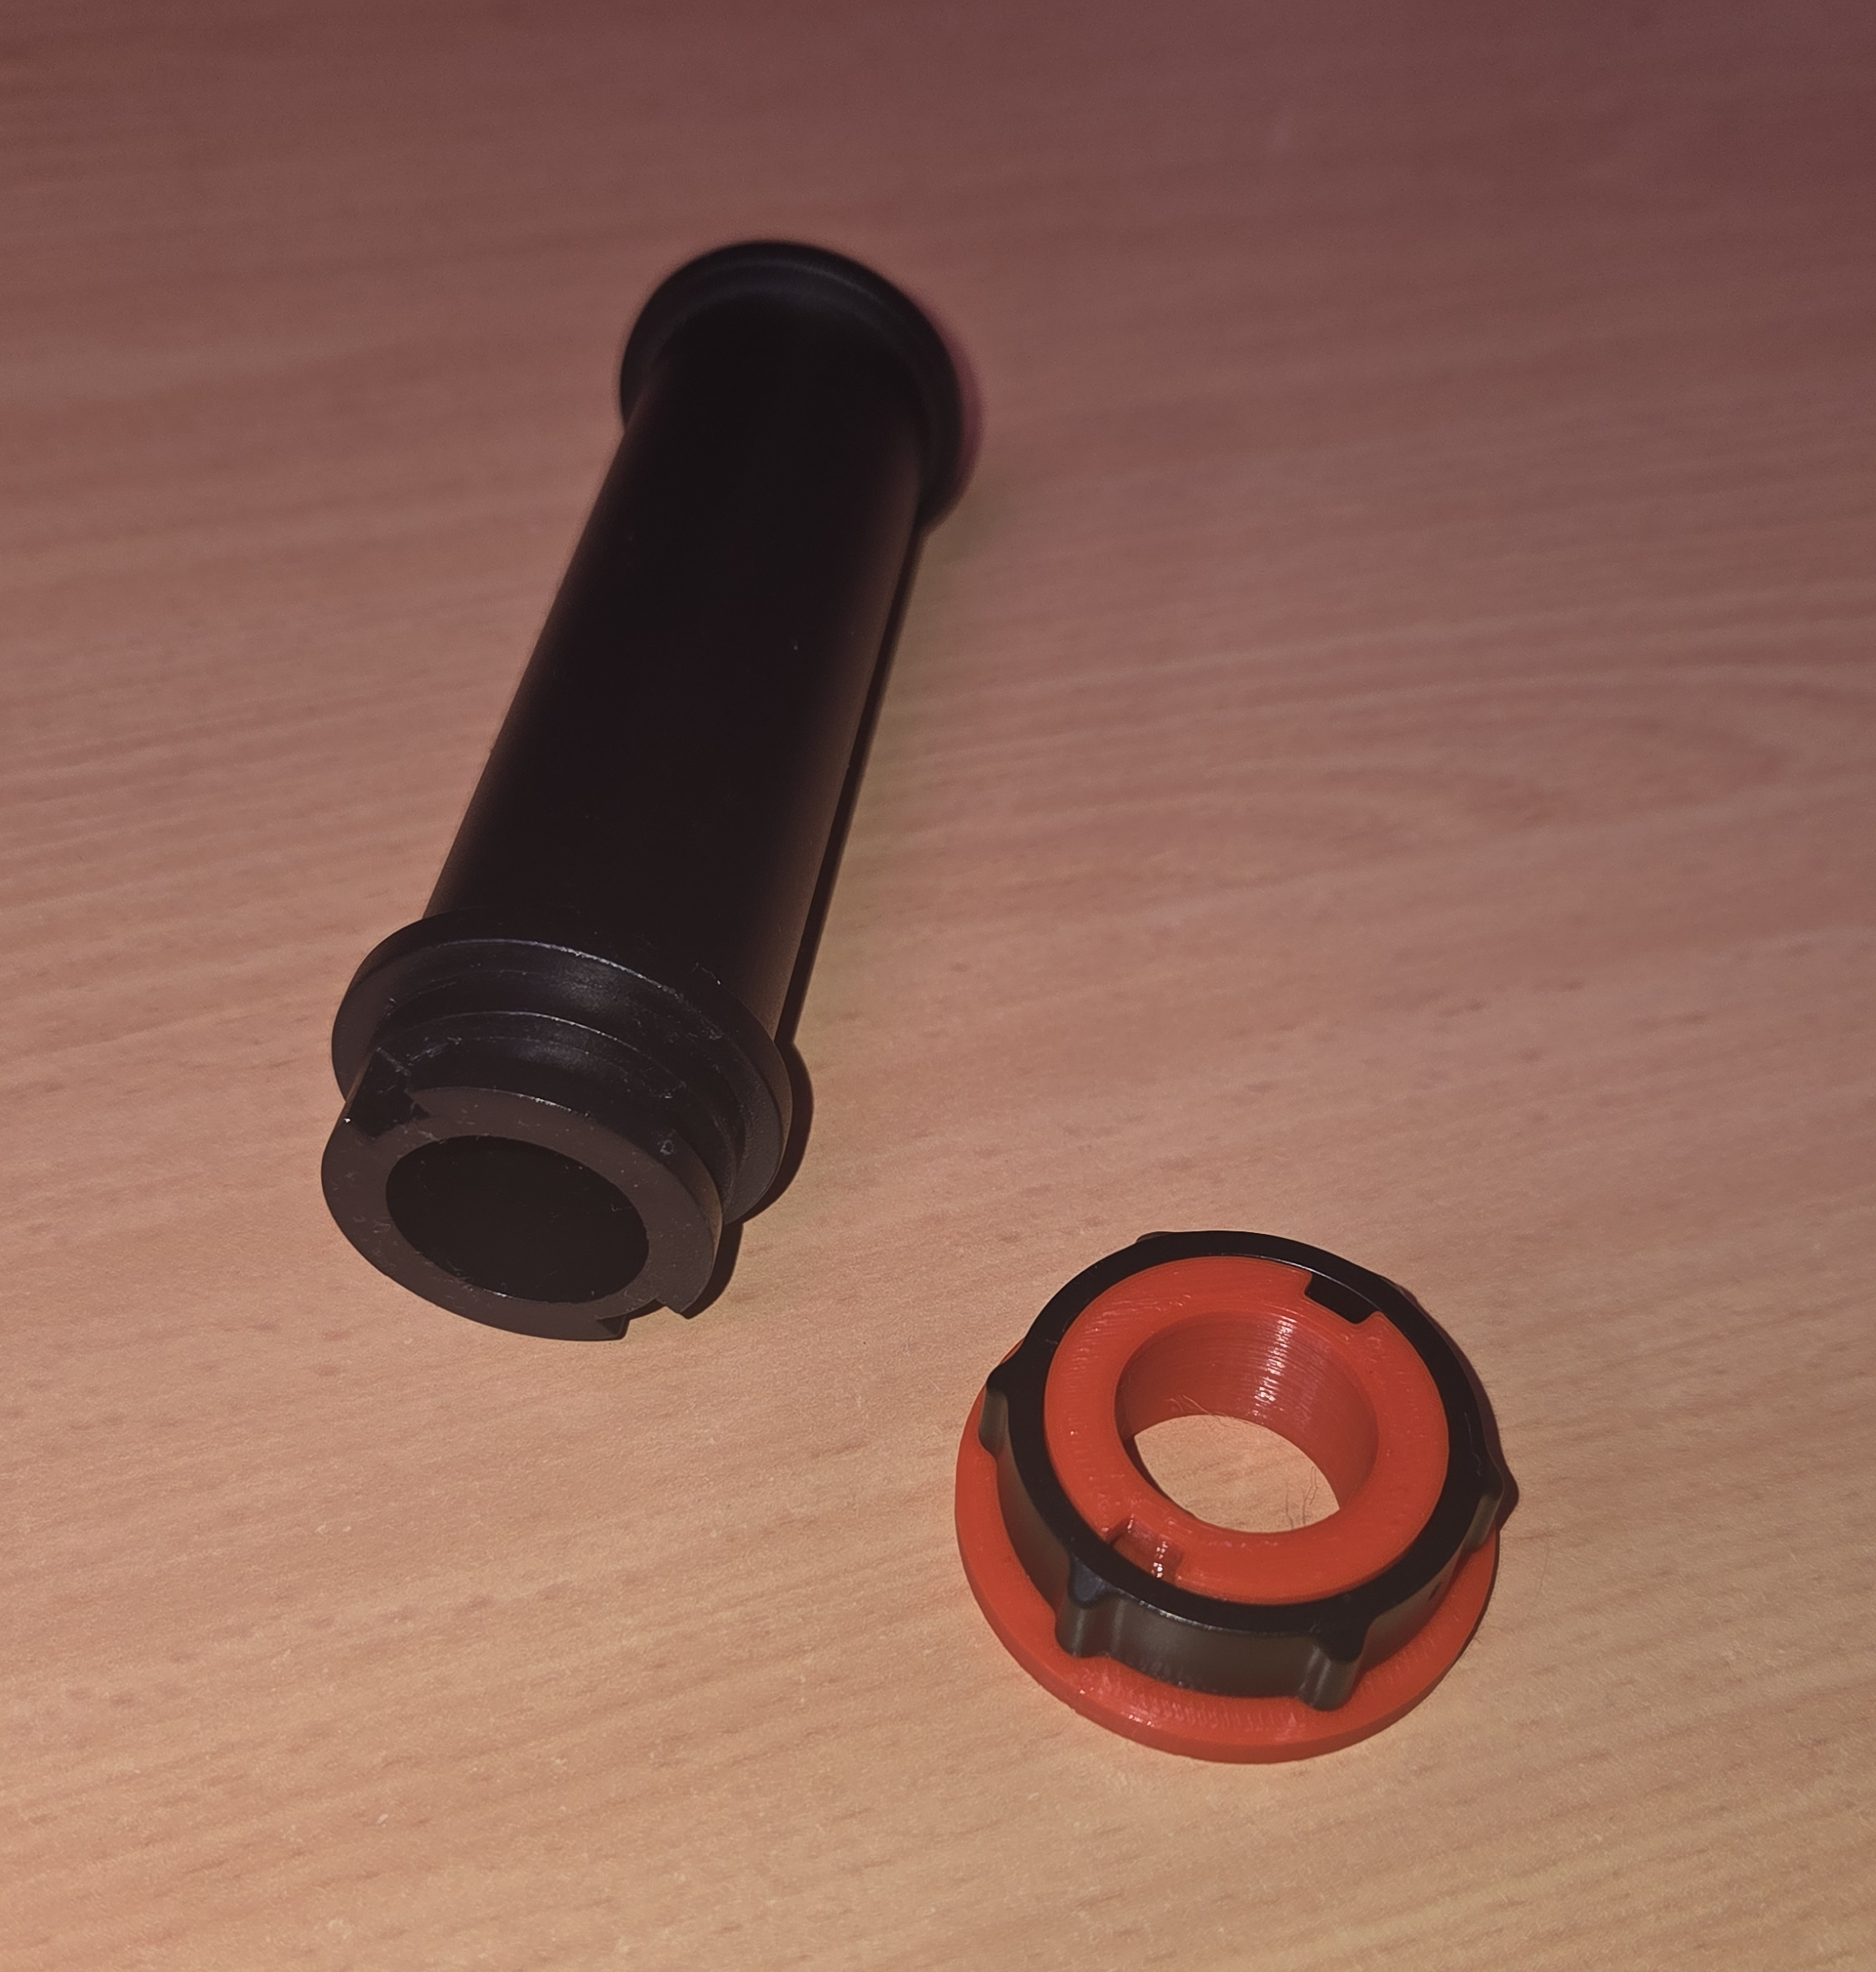
\includegraphics[width={\dimexpr\textwidth/2 - 6pt - 1pt\relax}]{./Images/OrignalMount3DPrintedConcept.png}
	\caption{Twist Lock CAD design recreation of the original \Printername\;interface}\label{fig:OrignalDesignConcept}
\end{figure}


\begin{table}[H]
\caption{Twist Lock Pros and Cons table}\label{tab:ProsandCons_TwistLock}
\begin{tabularx}{\textwidth}{|X|X|}

	\hline
	Pros & Cons \\
	\hline
	\begin{itemize}
		\item Proven Design
		\item Inner hole radius can be decreased to increase strength. 
	\end{itemize}& \begin{itemize}
	\item Requires support
	\item Required accurate tolerance between nut and attachment.
\end{itemize} \\
	\hline
\end{tabularx}   
\end{table}

%---------L bracket-------------------------
%-------------------------------------------
\paragraph{L-Bracket}
The second concept would be to replace the original L-Bracket on the \Printername\;with a 3D printed part. It would reuse the bolt holes of the original bracket. This design would  take advantage of the original printer interface and can be removed via unbolting. A representation of the design can be seen in Fig.\ref{fig:LAssembilyCAD}  

\begin{figure}[tbh!]
	\centering
	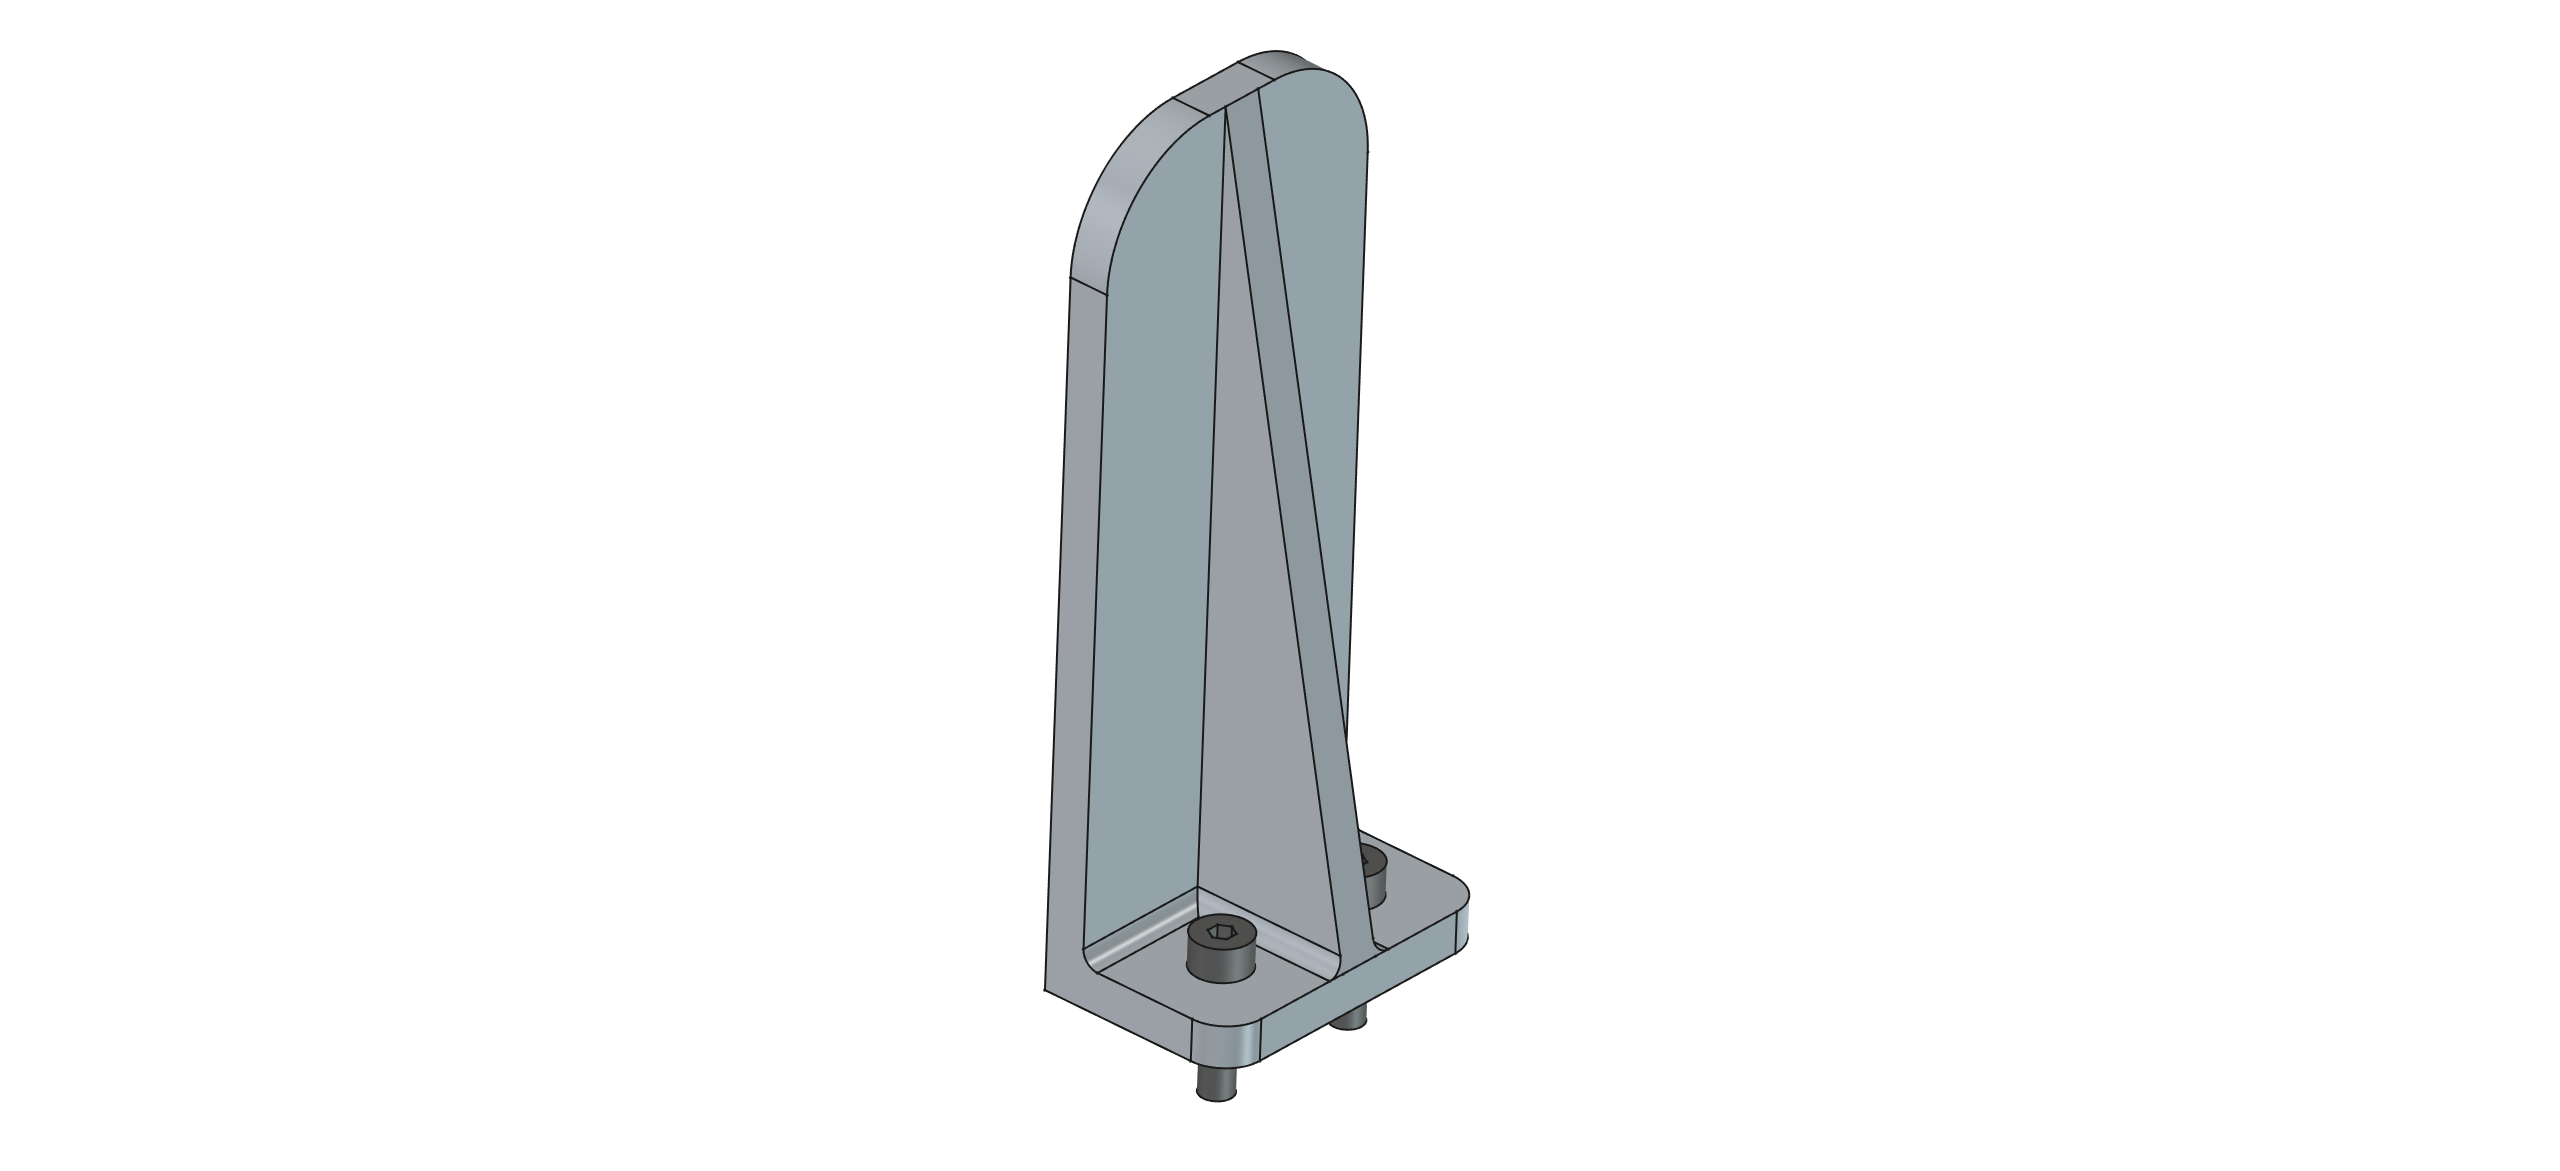
\includegraphics[width={\dimexpr\textwidth - 6pt - 1pt\relax}]{./Images/BoltAssembily_CAD100mm.png}
	\caption{L-Bracket Design CAD model}\label{fig:LAssembilyCAD}
\end{figure}
\begin{table}[H]
	\caption{L-Bracket Pros and Cons table}\label{tab:ProsandCons_LBracket}
\begin{tabularx}{\textwidth}{|X|X|}
	\hline
	Pros & Cons \\
	\hline
	\begin{itemize}
		\item Sturdy
		\item Possible to modify geometry for additional strength
		\item Could place 2D cosmetic design on flat face. 
		
	\end{itemize}& \begin{itemize}
		\item If printed with the filament mount in one print, would require significant support. 
		\item If printed in two parts, would need to consider additional attachment method
		\item Relatively large print if the filament mount is included.
	\end{itemize} \\
	\hline
\end{tabularx}  
\end{table}


\subsubsection{Routing Guide Design}
%---------Fixed Pulley Guide lock-------------------------
%-------------------------------------------
\paragraph{Fixed Pulley Guide} The first concept that was considered was to recreate the original spool shape, as can be seen in Fig.\ref{fig:Spool3Ddesign}.  To reduce filament friction and to make it more printable, the spool has a round inner surface. I have also considered two designs for the spool, the full rotation and the half rotation. The full rotation will be needed if the attachment is not fixed axially, like the Twist Lock interface. The half rotation can be used if it is, like the L-Bracket. 

\begin{table}[H]
	\caption{Fixed Pulley Guide Pros and Cons table}\label{tab:ProsandCons_FixedPullyGuide}
\begin{tabularx}{\textwidth}{|X|X|}
	\hline
	Pros & Cons \\
	\hline
	\begin{itemize}
		\item Standard Design
		\item Sturdy
		\item Can be used with both Printer interfaces. 
		
	\end{itemize}& \begin{itemize}
		\item Would require some support to be used.
		\item Large print
		\item Need to consider the friction between the filament and the guider
		
	
	\end{itemize} \\
	\hline
\end{tabularx}  
\end{table}
\begin{figure}[tbh!]
	\centering
	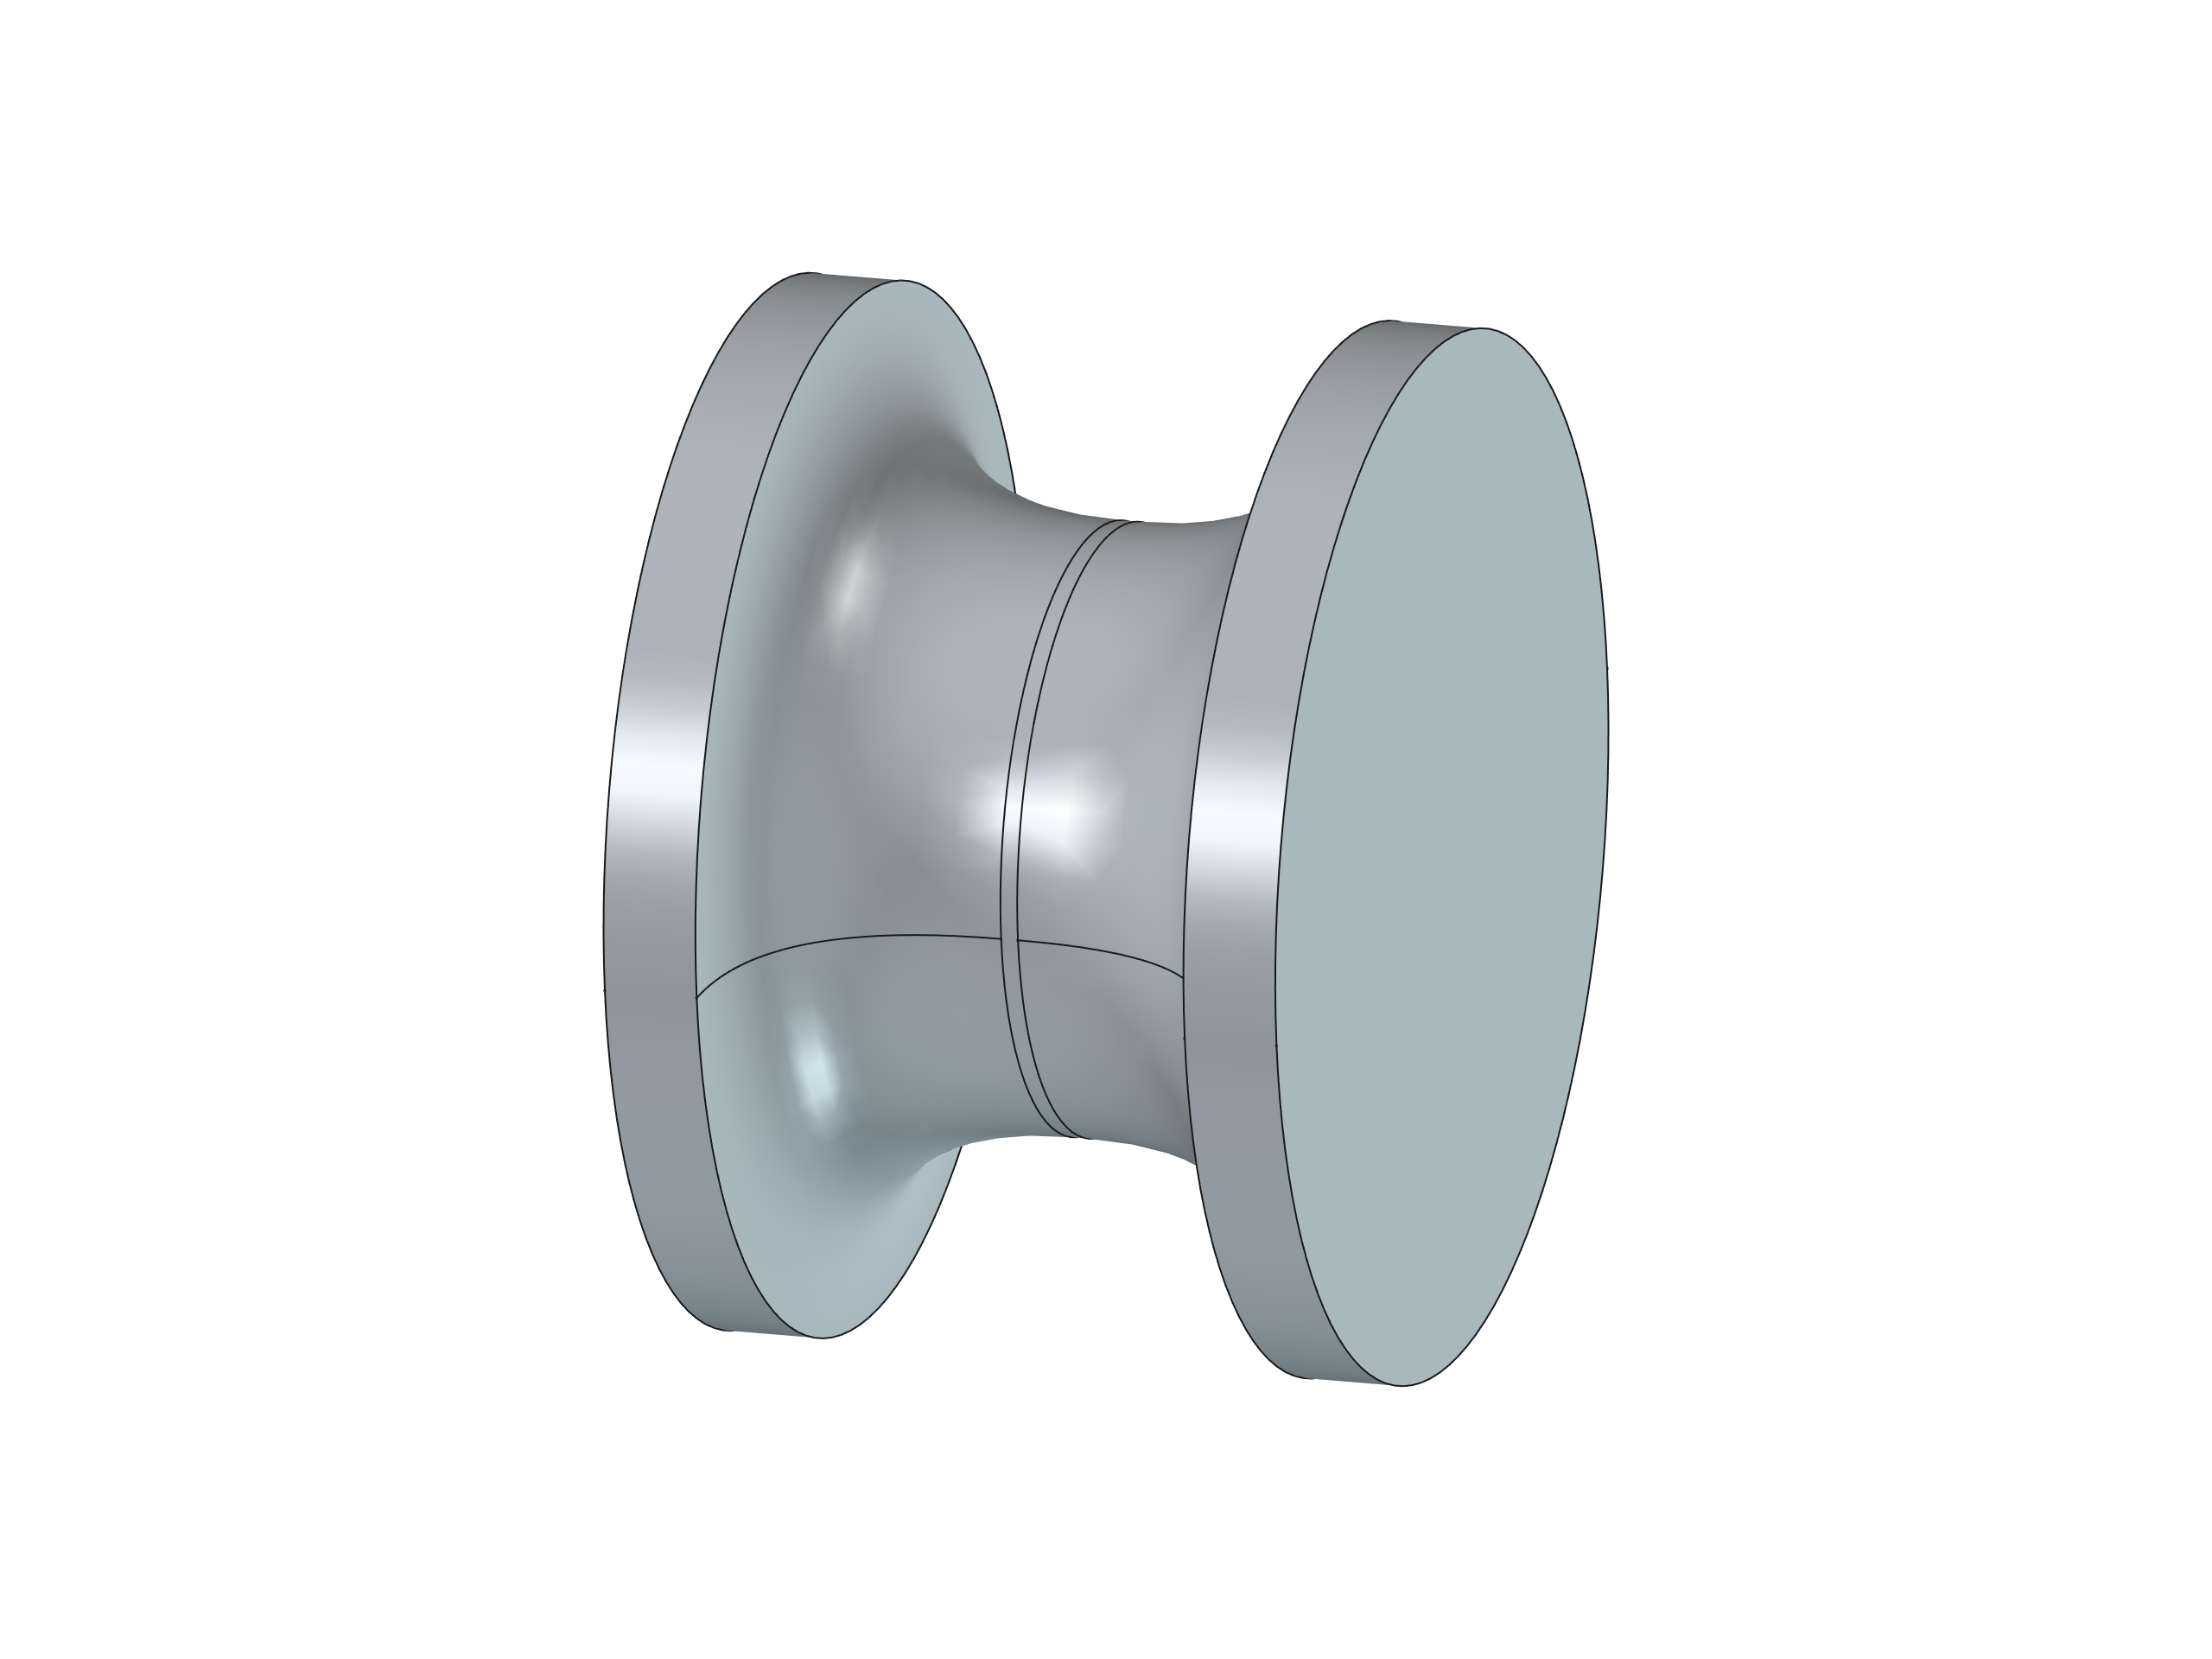
\includegraphics[width={\dimexpr\textwidth/2 - 6pt - 1pt\relax}]{./Images/SpoolFullRev.png}
	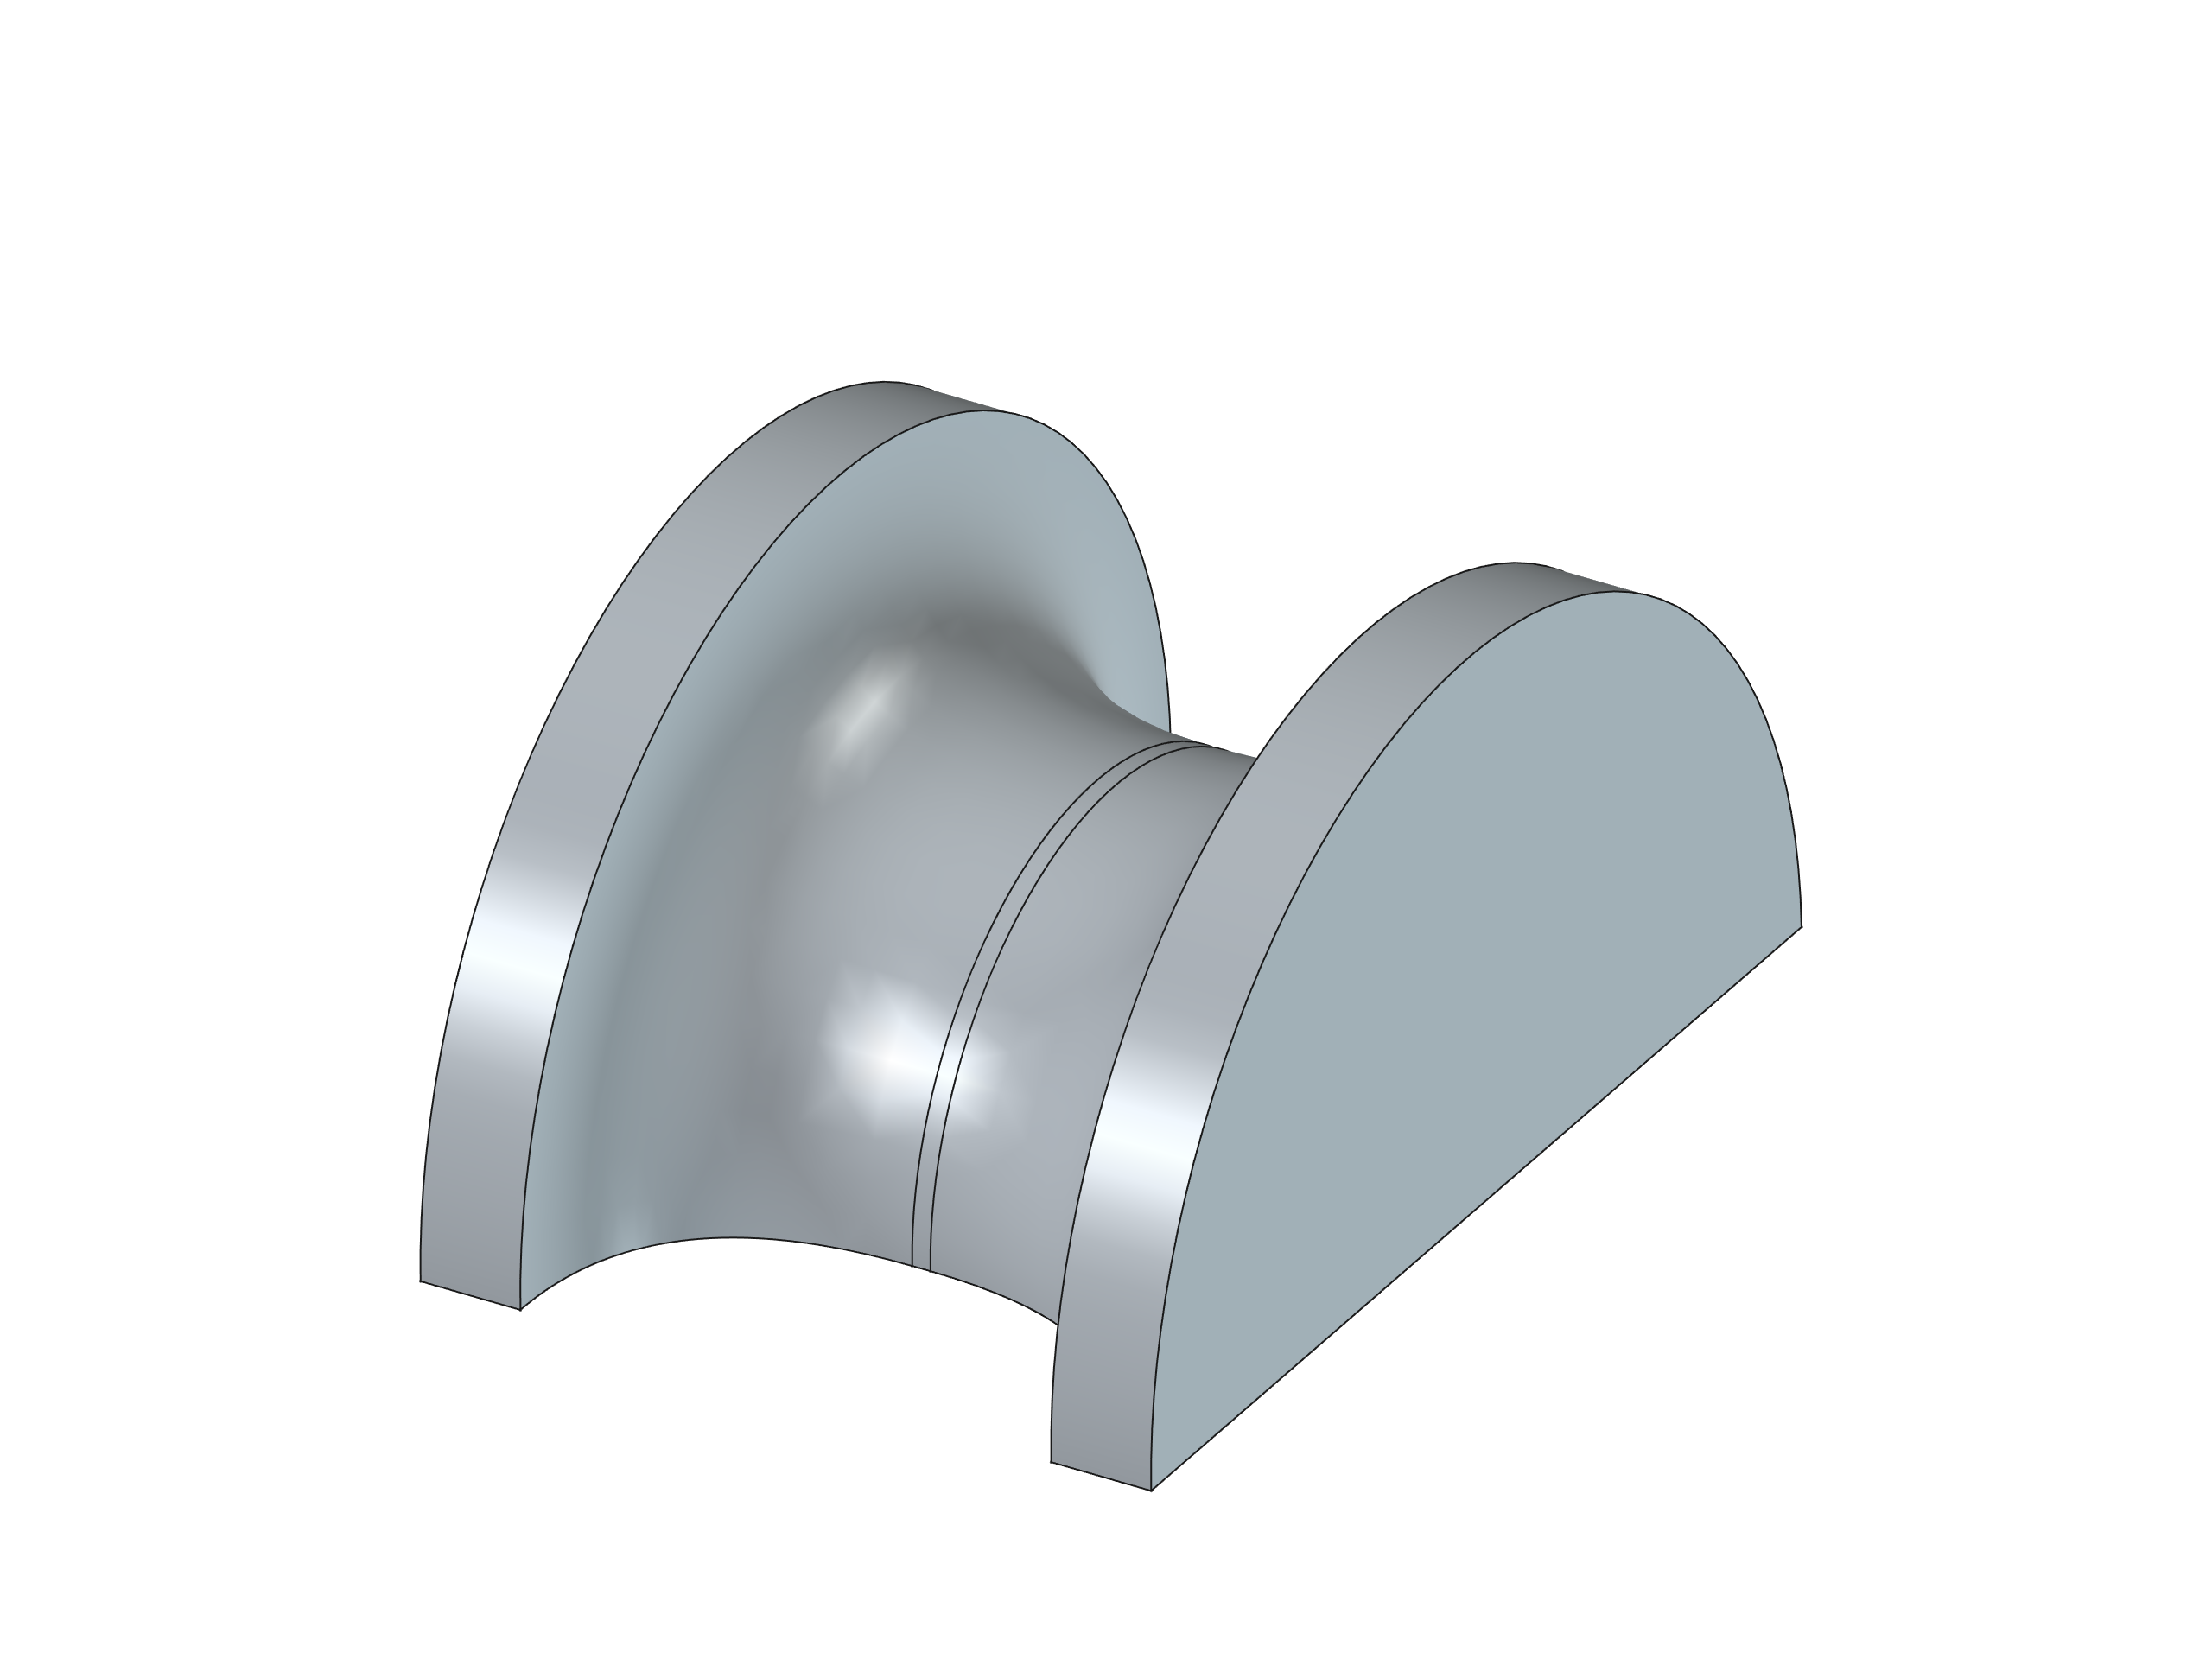
\includegraphics[width={\dimexpr\textwidth/2 - 6pt - 1pt\relax}]{./Images/SpoolHalfRev.png}
	\caption{Fixed Pulley Guide CAD Design}\label{fig:Spool3Ddesign}
\end{figure}

\paragraph{Pulley Guide} A technique that I have yet to implement in my 3D designs is the use of bearings and I think it could potentially be applicable for this project. An image of the design can be seen in Fig.\ref{fig:SpoolBearing3Ddesign}. The design would be the same as the full-revolution fixed pulley, however with a bearing in the centre to allow for free rotation. The ball bearing considered would be a standard 608SS bearing. This would be sourced from an old skateboard that has ABEC-7 608ZZ bearings. A hex bolt would go through the centre of the spool and act as an axle, attaching to the two bearings and attaching to the frame mount. The load would be concentrated at the axle-to-frame-mount interface. The frame mount would have to take the cantilever force of the spool. To ensure this does not fail, testing would need to be done. 
\begin{table}[H]
	\caption{Pulley Guide Pros and Cons table}\label{tab:ProsandCons_PullyGuide}
\begin{tabularx}{\textwidth}{|X|X|}
	\hline
	Pros & Cons \\
	\hline
	\begin{itemize}
		\item Common Design
		\item Sturdy Spool
		\item Minimal friction on filament
	\end{itemize}& \begin{itemize}
		\item Would require semi-complex assembly, nut, bolt, bearings etc. 
		\item Need to interface the bolt with the Frame mount design. Allowing the axle to be clamped to the Frame mount design while not touching the spool. 
		\item Would require a sturdy Frame Mount Design as there will be a strong cantilever force on the bolt.
	\end{itemize} \\
	\hline
\end{tabularx}  
\end{table}
\begin{figure}[tbh!]
	\centering
	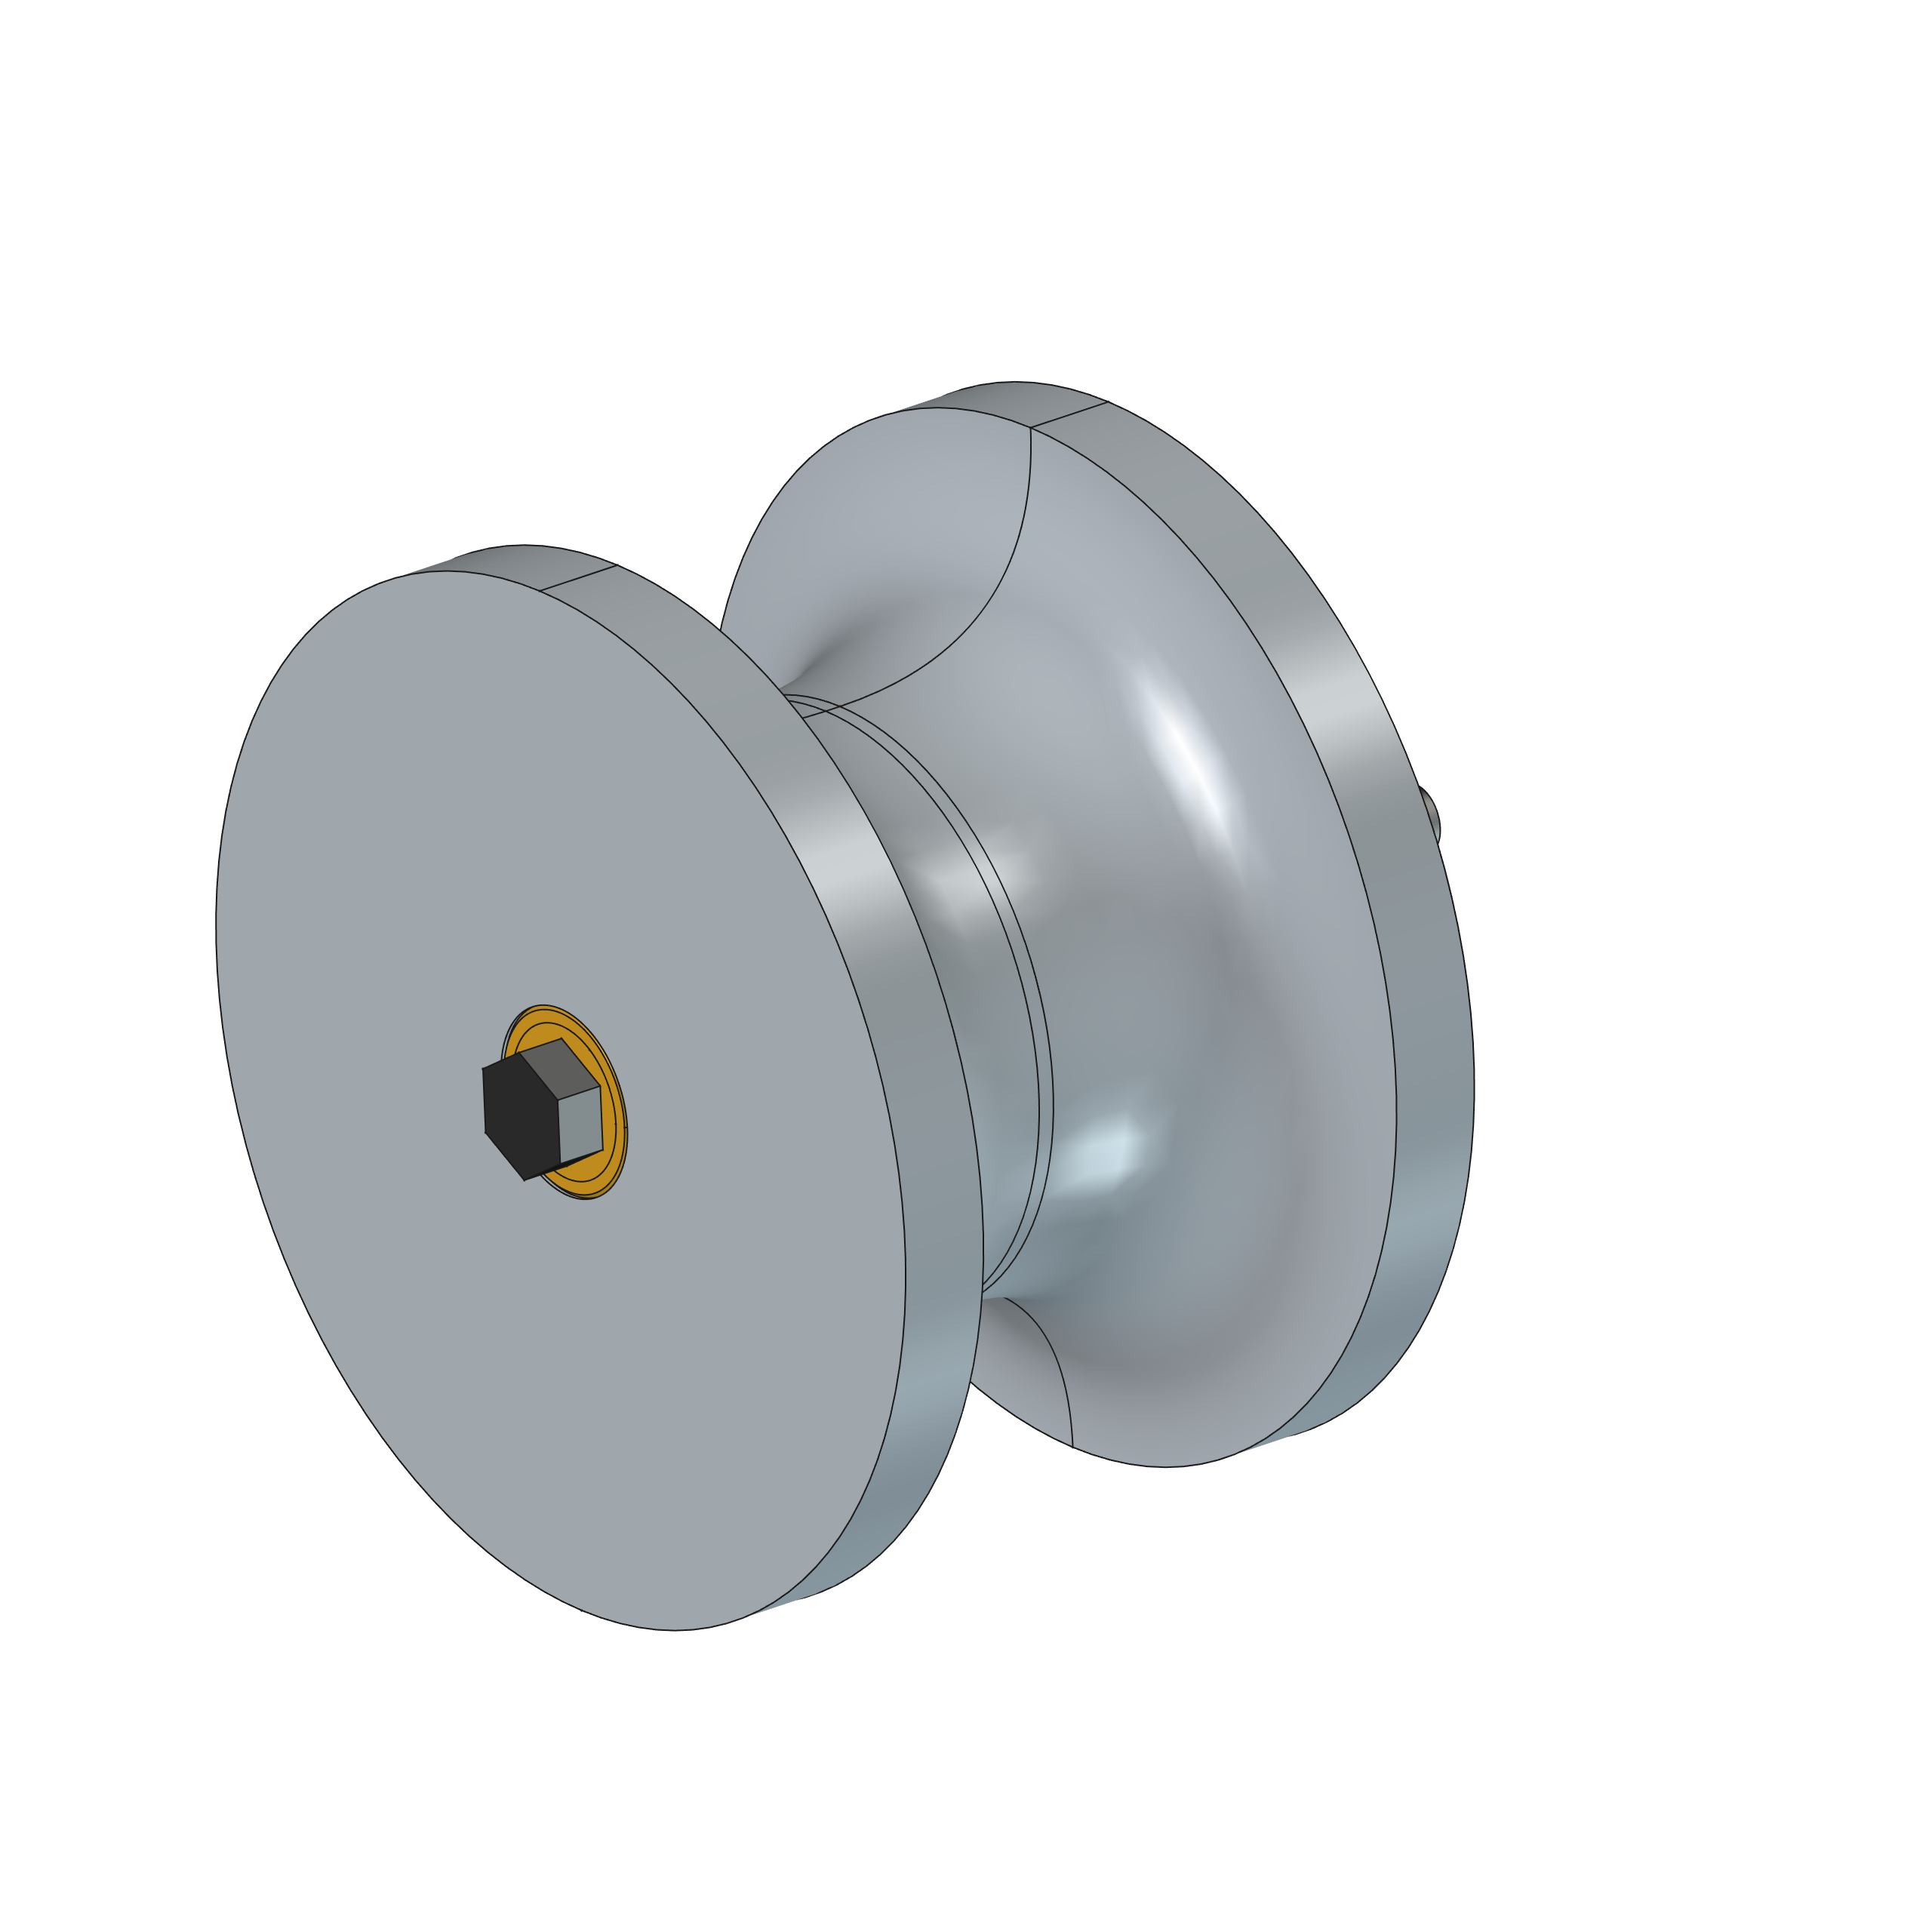
\includegraphics[width={\dimexpr\textwidth/2 - 6pt - 1pt\relax}]{./Images/SpoolBearingIso.png}
	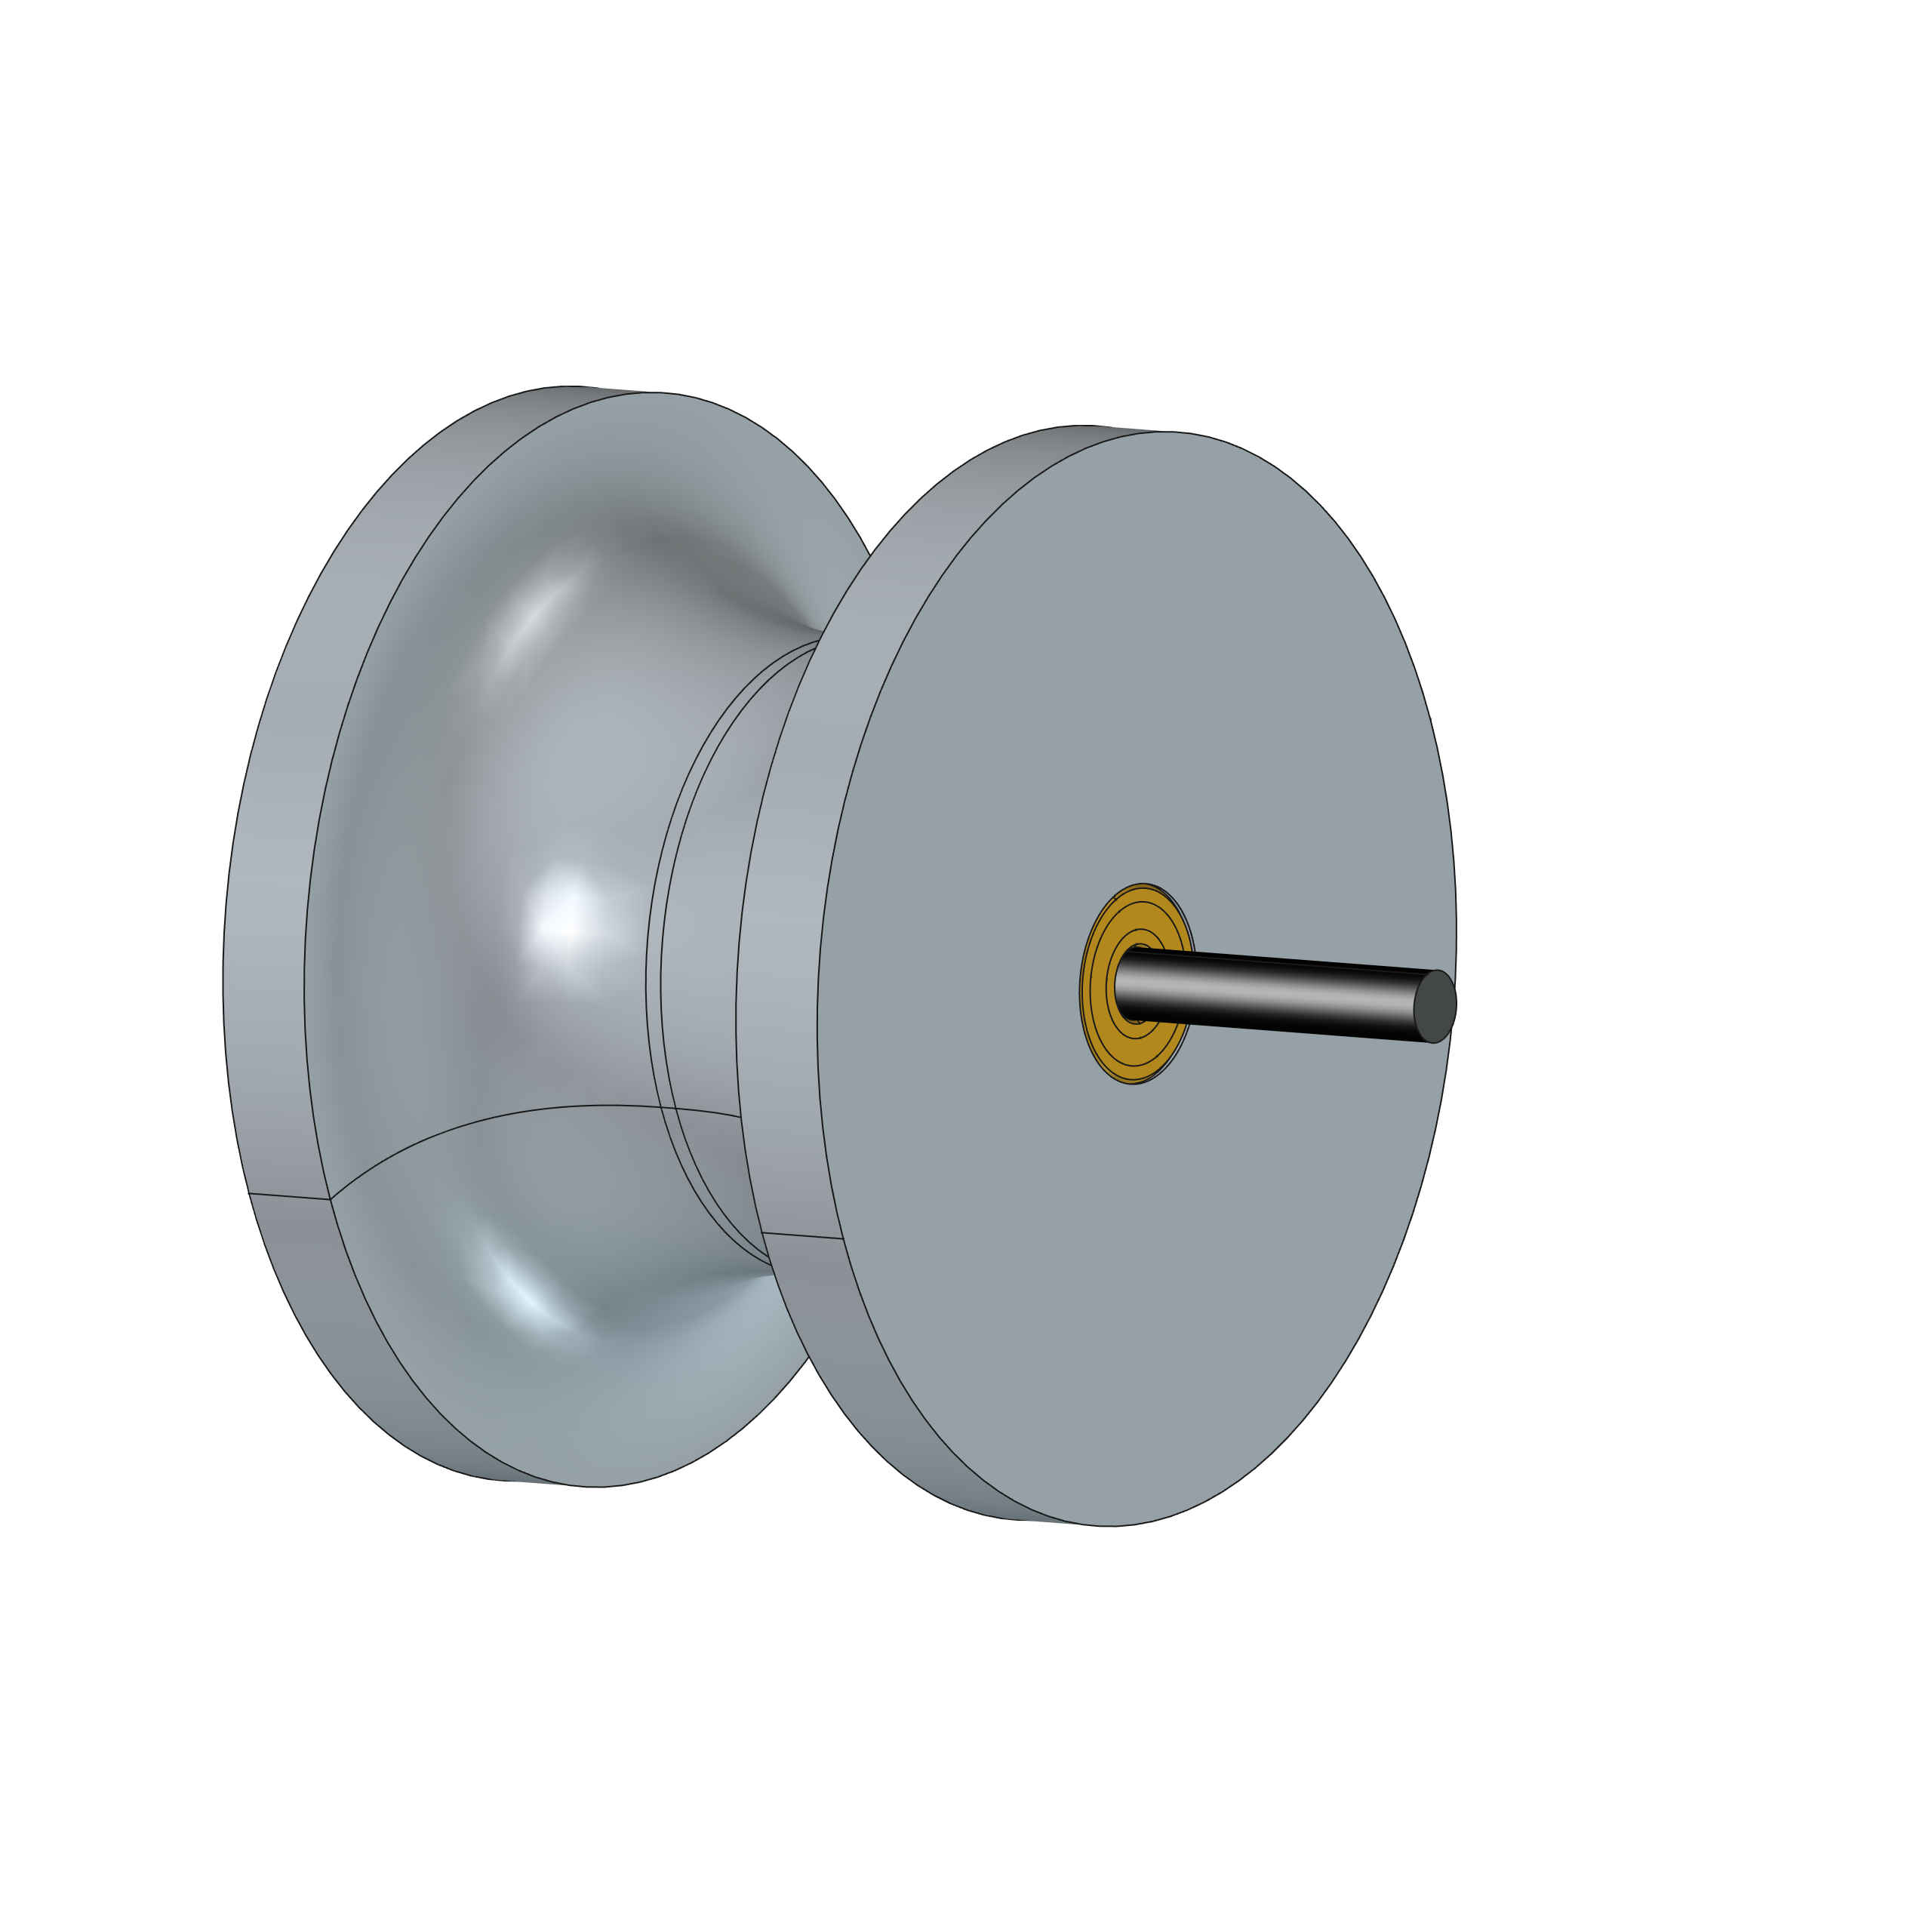
\includegraphics[width={\dimexpr\textwidth/2 - 6pt - 1pt\relax}]{./Images/SpoolBearingIso2.png}
	\caption{Pulley Guide CAD design}\label{fig:SpoolBearing3Ddesign}
\end{figure}
\paragraph{Bracket-Supported Tube} A tube could be implemented that could be guided by a 3D printed component. This would allow for a predefined path around the filament holder. A concept of the design can be seen in Fig.\ref{fig:Bracket-SupportTubeAssembily}. The red tube in the component would be a Bowden tube that would extend up to the top of the gantry frame. As the extruder would be moving relative to the Filament Guide, the tube cannot be directly attached to the extruder. The tube would need to be securely in place to ensure that the tube does not fall onto the extruder, or cause issues elsewhere. 

\begin{table}[H]
	\caption{Bracket-Supported Tube Pros and Cons table}\label{tab:ProsandCons_BracketSupportedTube}
	\begin{tabularx}{\textwidth}{|X|X|}
		\hline
		Pros & Cons \\
		\hline
		\begin{itemize}
			\item Minimal Friction on filament as the tube is designed for filament
			\item Filament cannot slip out of the tube
		\end{itemize}& \begin{itemize}
			\item Requires installation and secure installation of the tube.
			\item Tube cannot connect to extruder like a real Bowden Tube.
		\end{itemize} \\
		\hline
	\end{tabularx}  
\end{table}

\begin{figure}[tbh!]
	\centering
	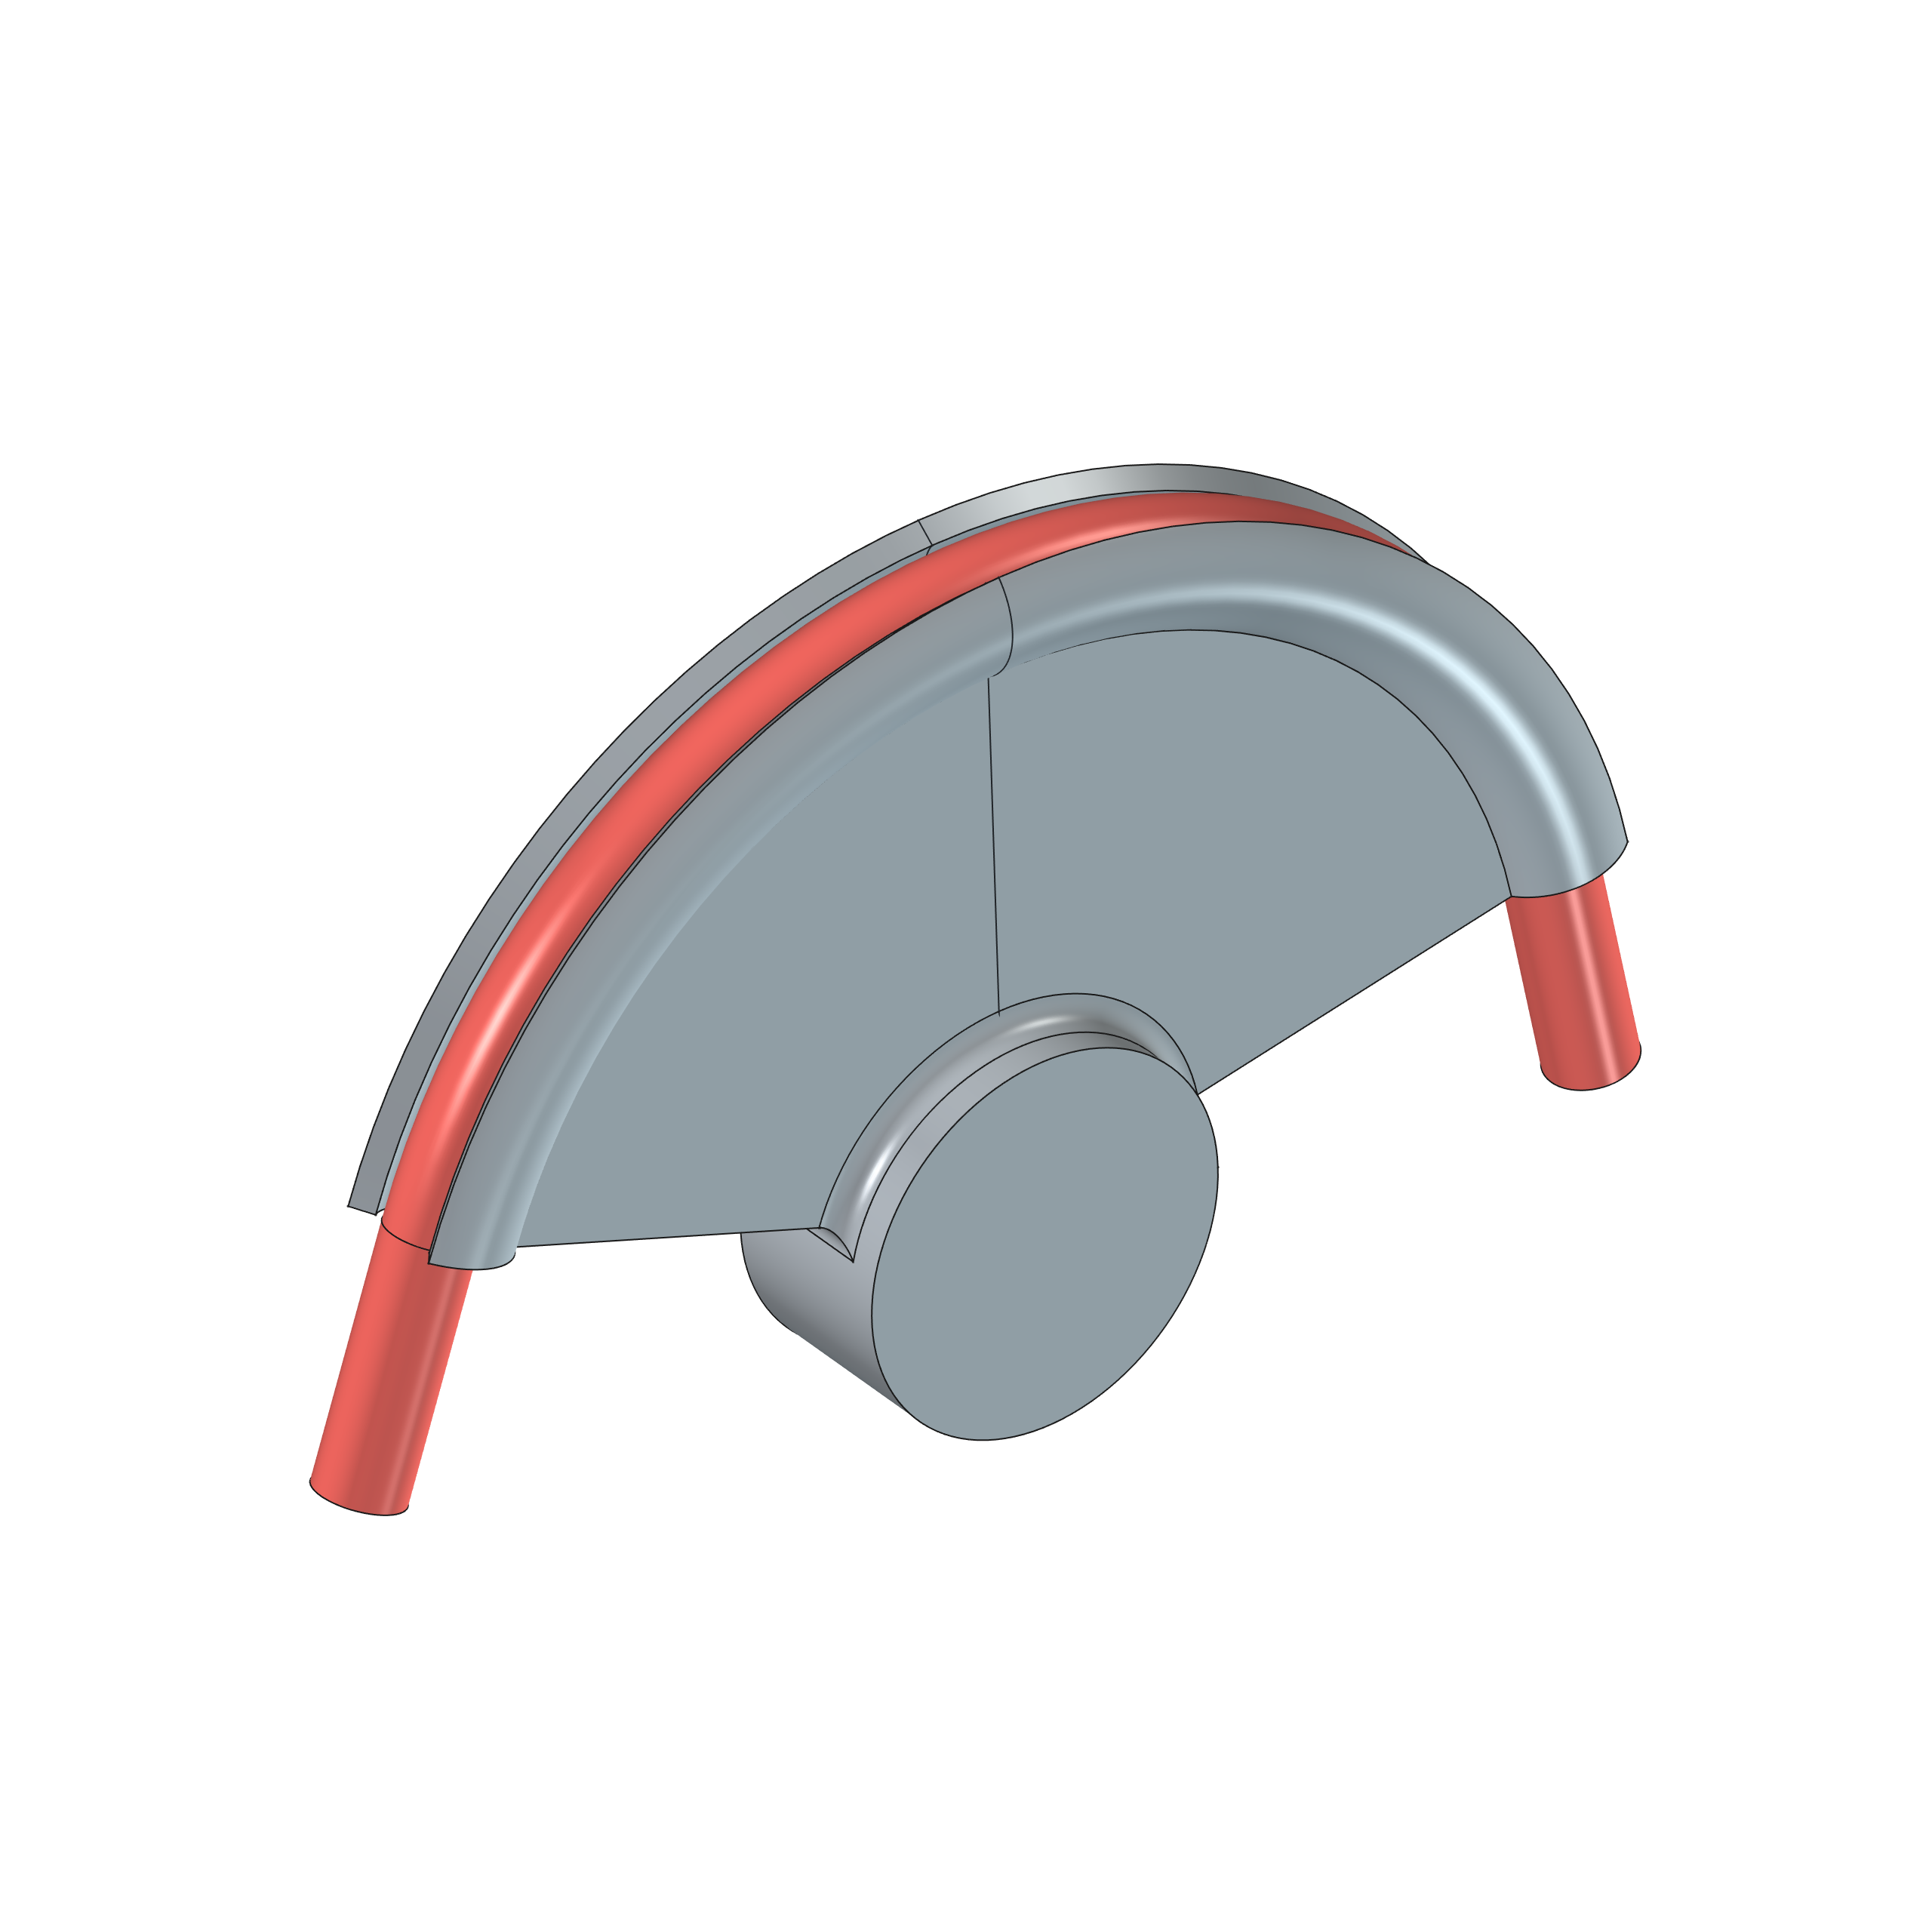
\includegraphics[width={\dimexpr\textwidth/2 - 6pt - 1pt\relax}]{./Images/TubeAssembilyDesign.png}
	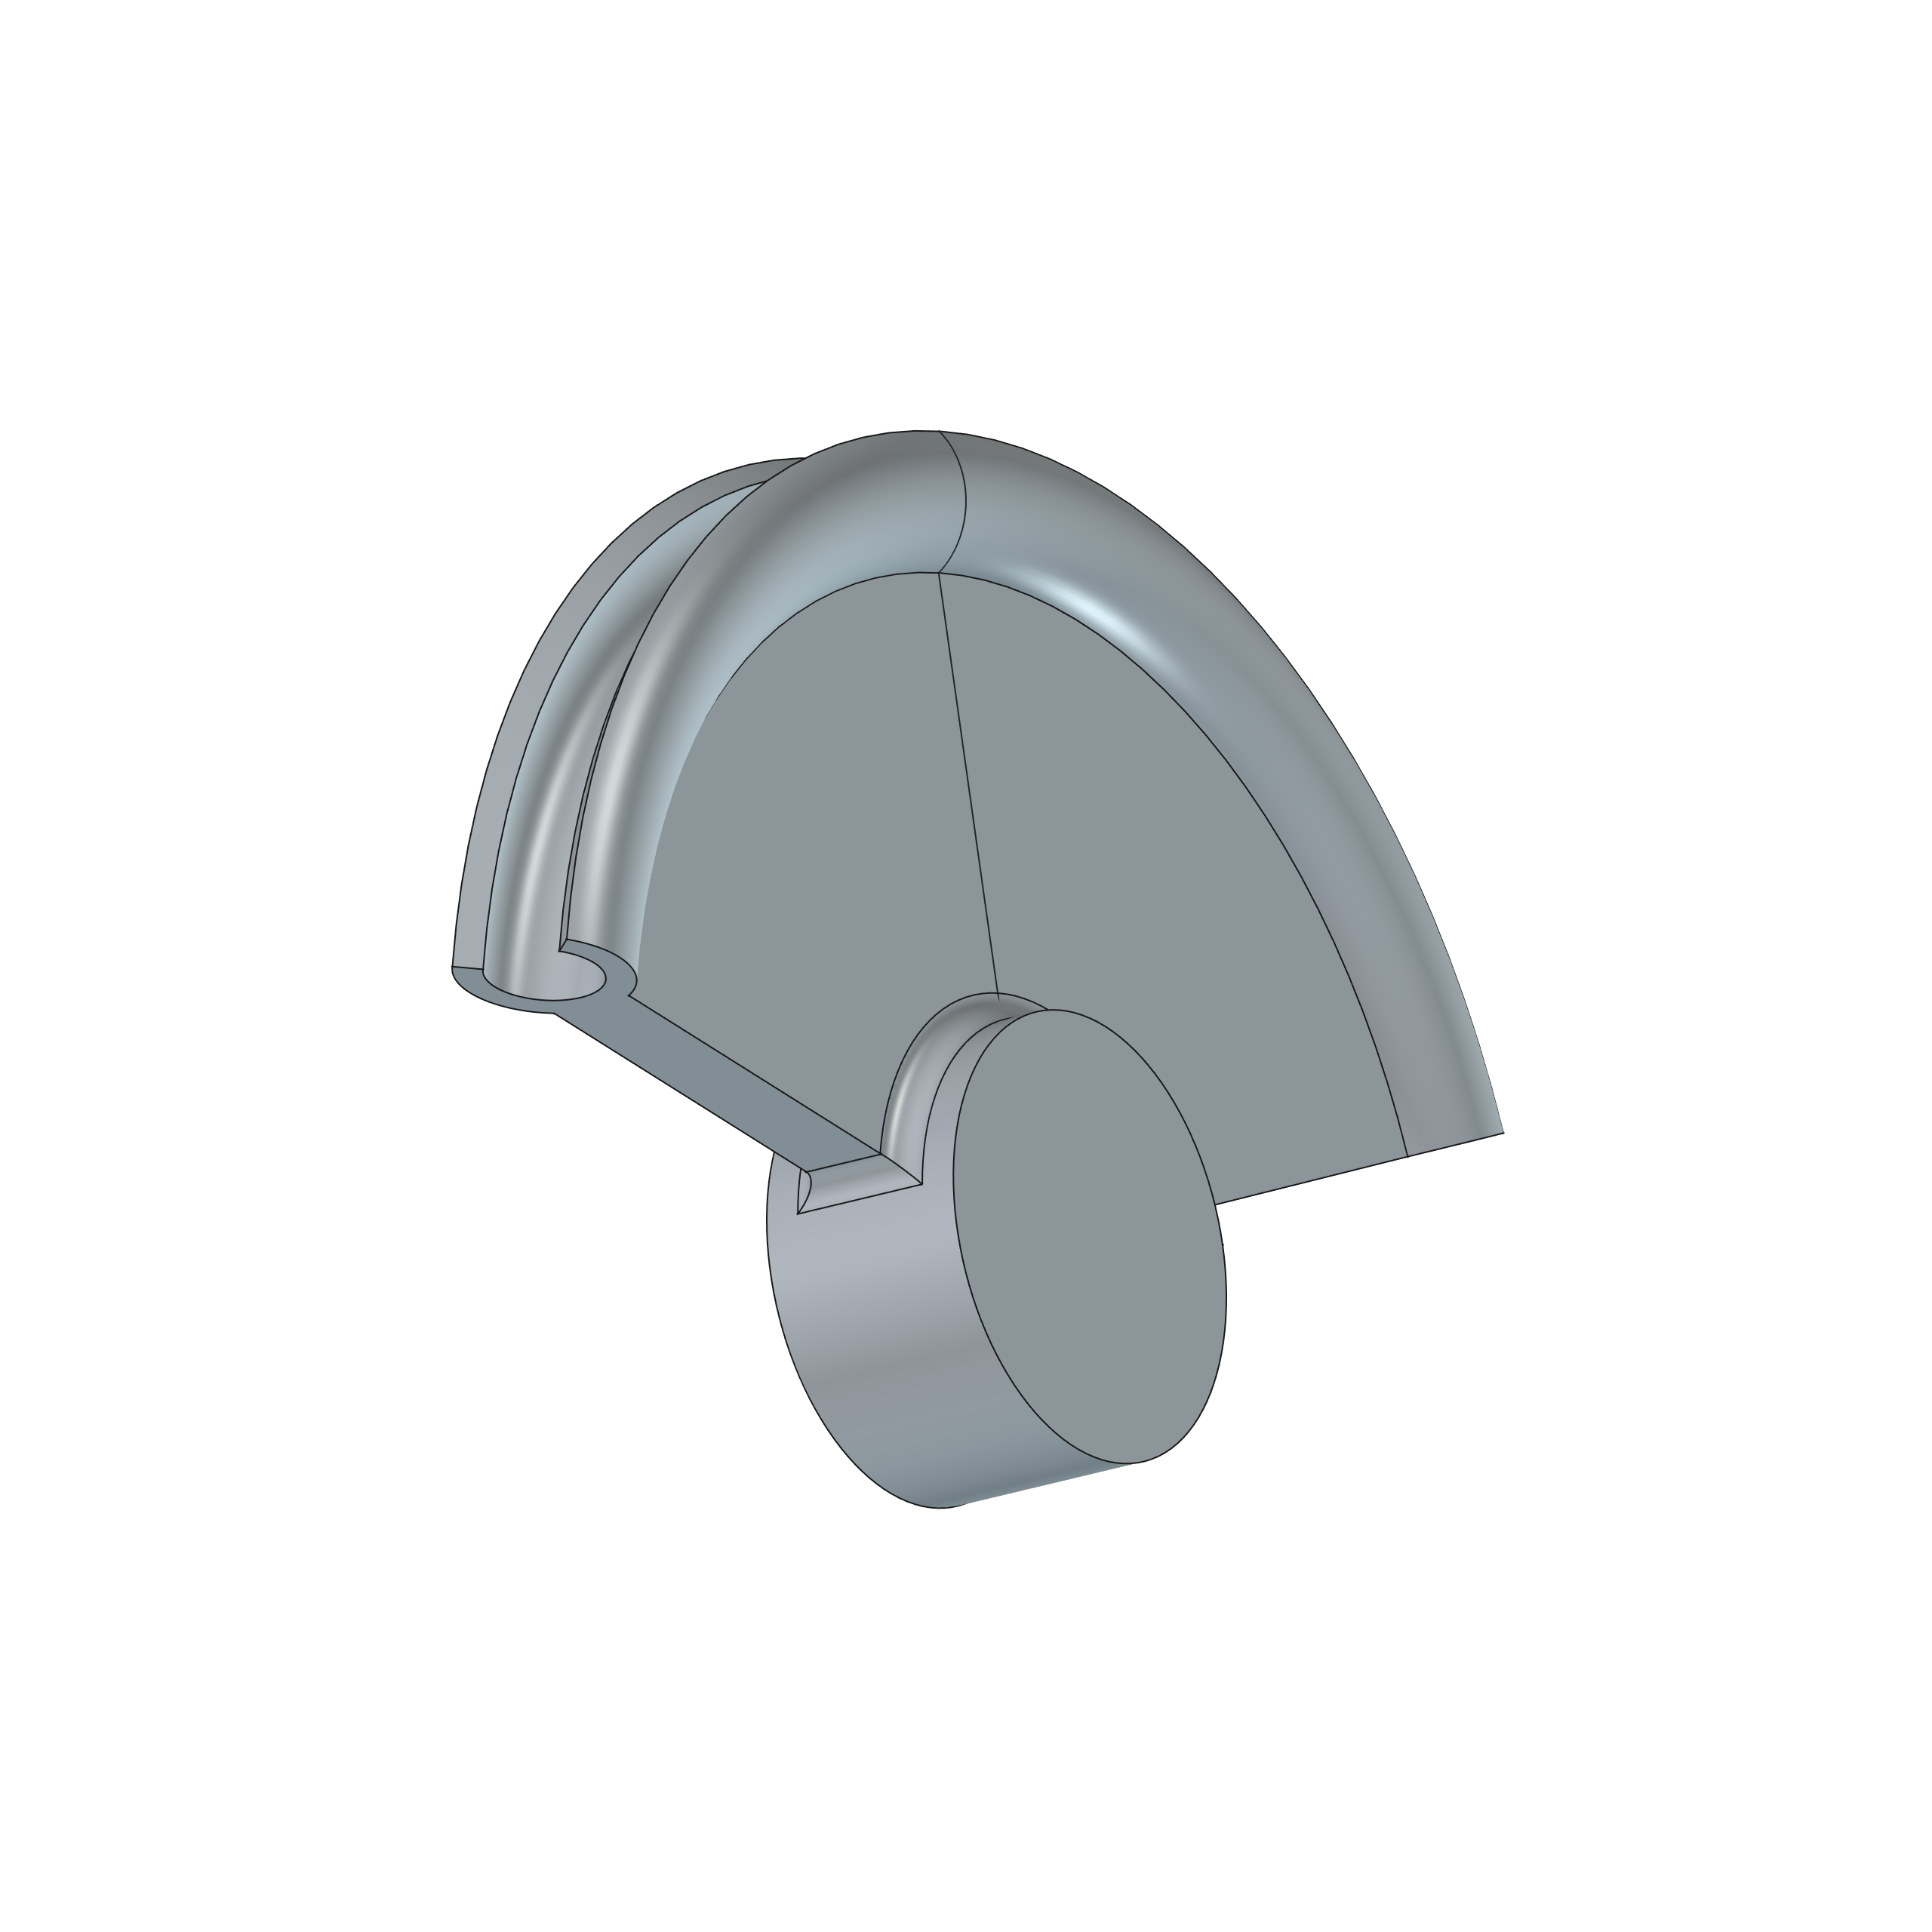
\includegraphics[width={\dimexpr\textwidth/2 - 6pt - 1pt\relax}]{./Images/TubeAssembilyDesign2.png}
	\caption{Bracket-Supported Tube CAD model}\label{fig:Bracket-SupportTubeAssembily}
\end{figure}


\subsubsection{Design Concepts Conclusion}

\paragraph{Routing Guide Design Choice} The Routing Guide Design was chosen first as this selection directly affects what frame mount is suitable.  When considering the Pros and Cons of each Routing Guide, the Fixed Pulley Guide was selected over the regular Pulley Guide and the Bracket-Supported Tube.  The Bracket-Supported Tube would be a complex design, requiring the tube to be held securely, if not the printer may be damaged by the tube. Without the tube, the design is essentially the fixed pulley design. As for the fixed vs regular pulley system, the advantage of the bearings would be to reduce the friction on the filament. I do not think the friction will be an issue, if required, the filament may be sanded to reduce friction. Considering these factors, the fixed pulley has been selected. 

\paragraph{Frame Mounting Choice} When comparing the Twist Lock, to the L-Bracket, the Twist Lock has been shown to be a standard design choice. To change between the Twist Lock, back to the original filament it requires minimal effort. The Routing Guide that was selected does not require a fixed axes so the Twist Lock is acceptable. The L-Bracket and the fixed pulley design would be a very large design if printed together. I would also be concerned with the strength of the L-Bracket, as it would be a tall and narrow. So for these reasons, I have selected the Twist Lock. 

\begin{figure}[tbh!]
	\centering
	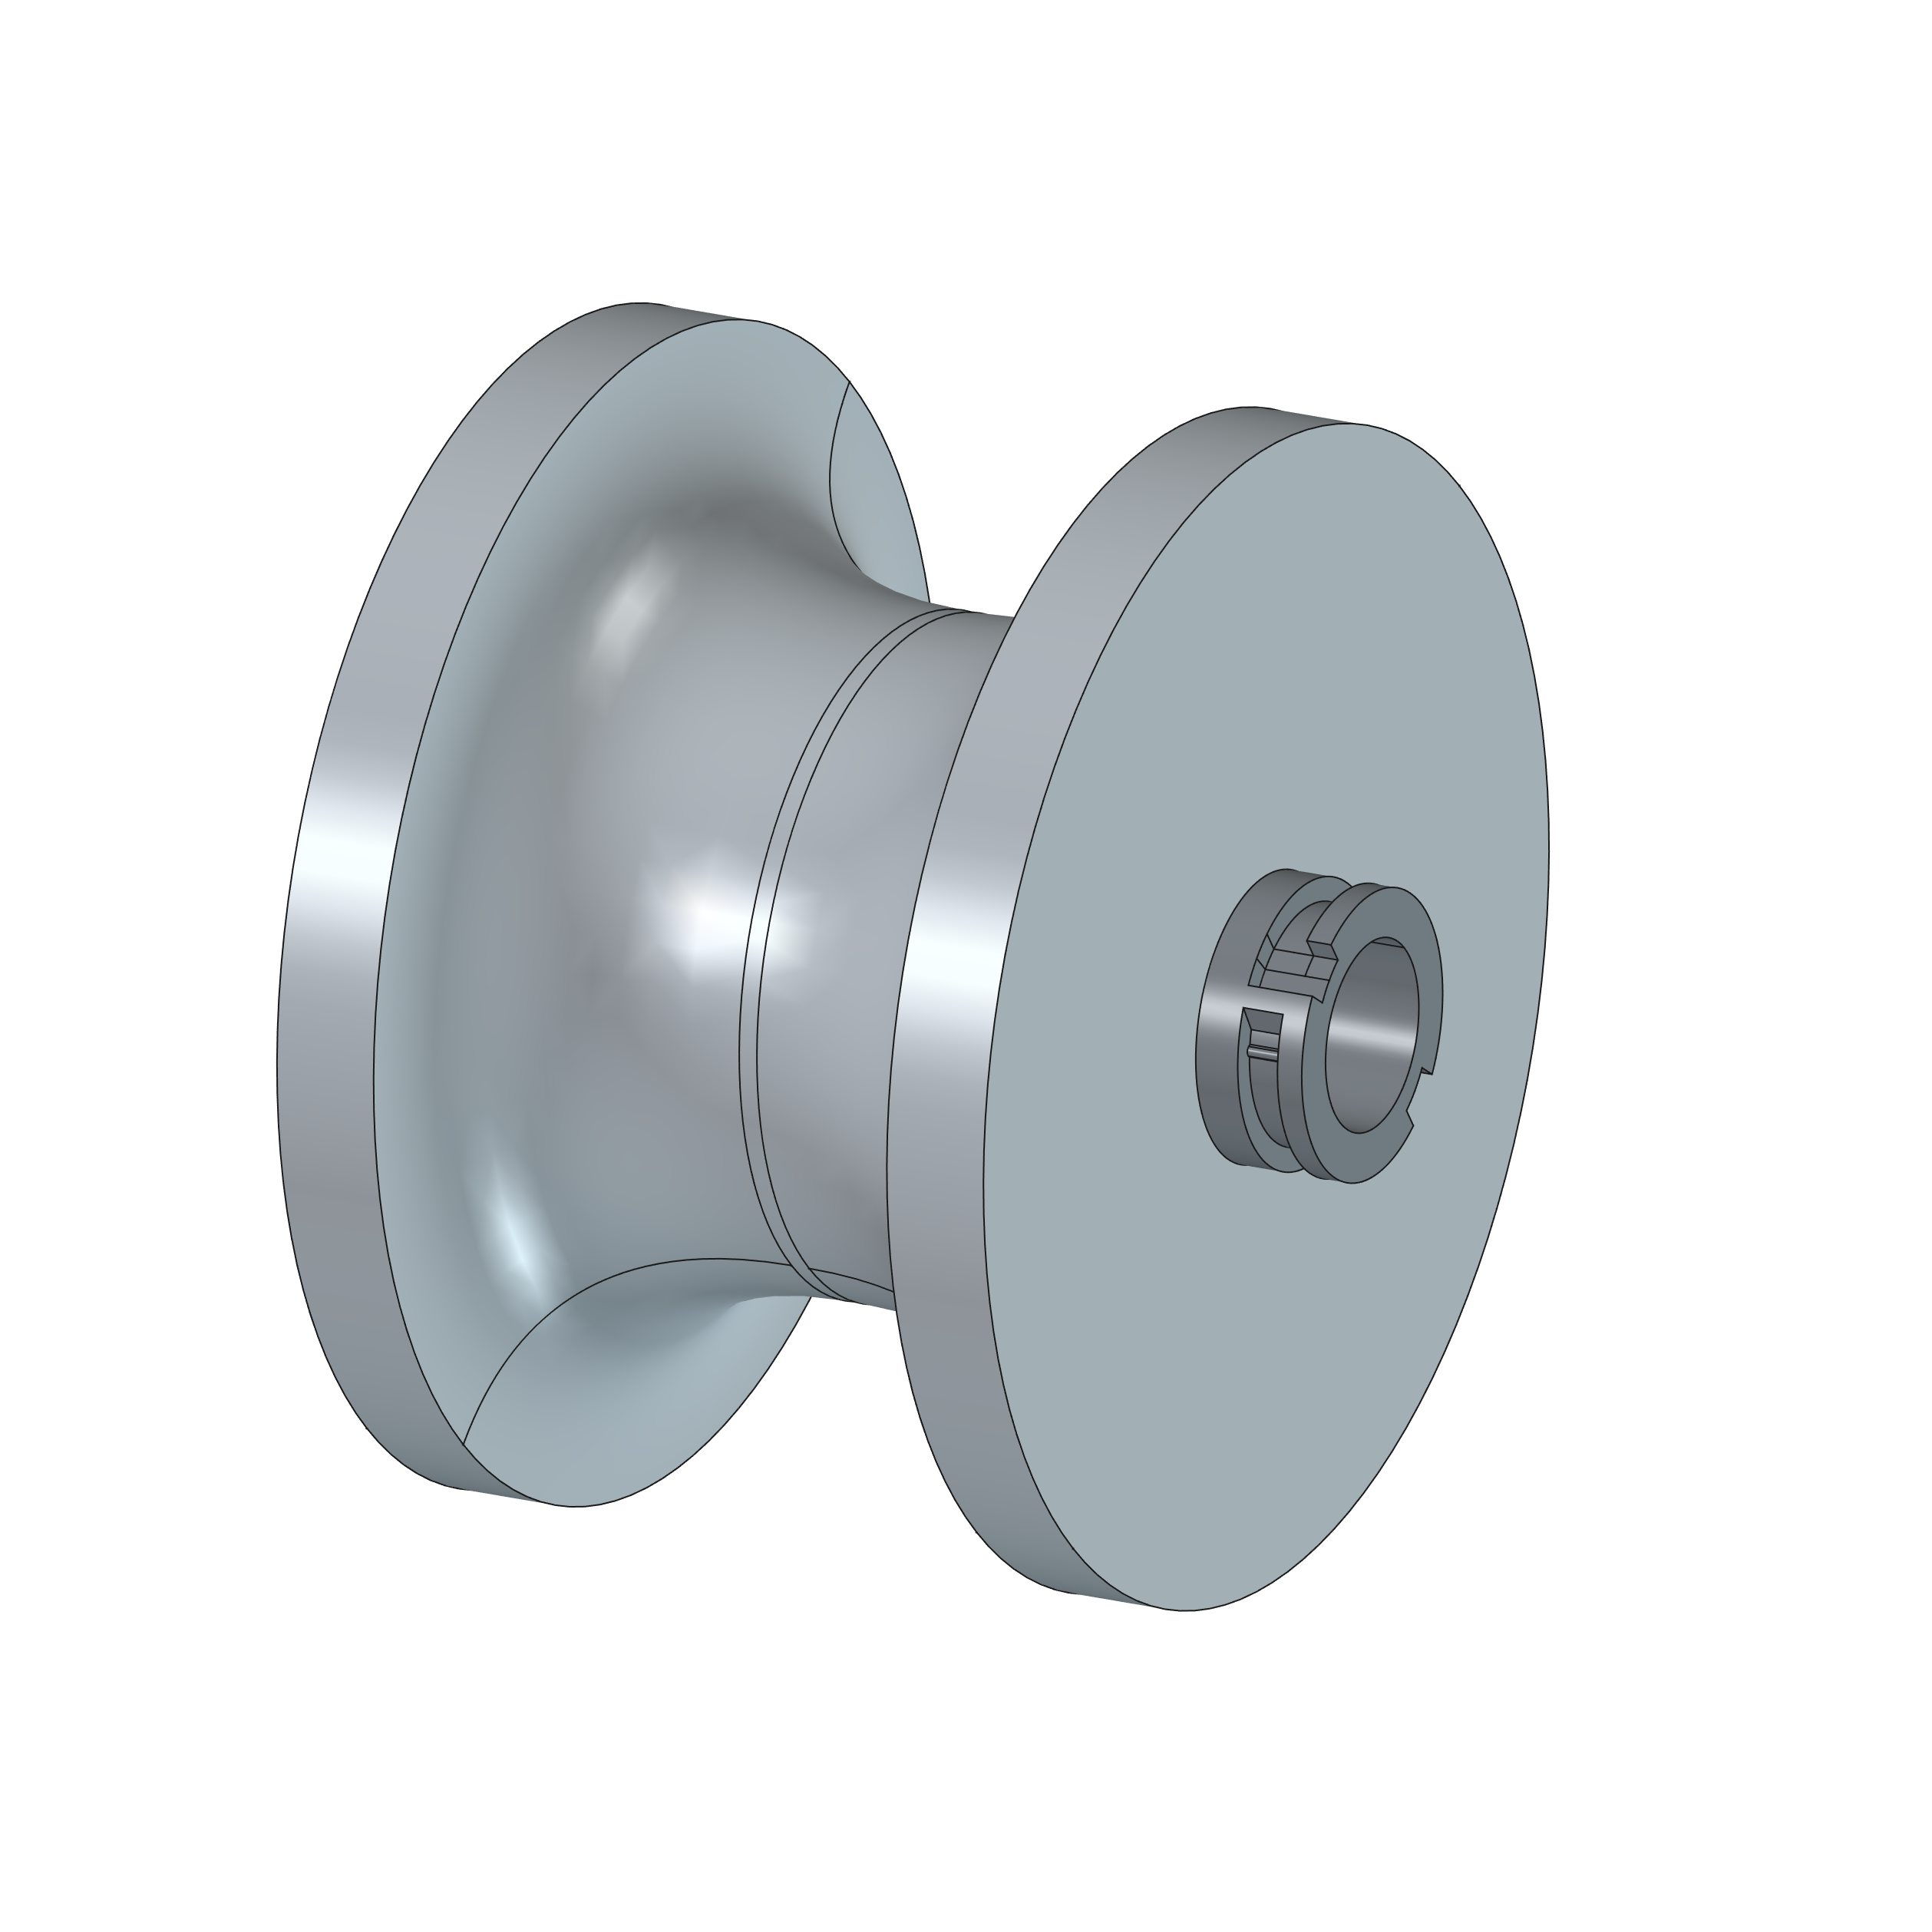
\includegraphics[width={\dimexpr\textwidth/2 - 6pt - 1pt\relax}]{./Images/Design1TwistLock_Spool.png}
	\caption{Design concept conclusion selection}\label{fig:Design1TwistLock_Spool}
\end{figure}
\paragraph{Design Concepts Conclusion} The final selection that was picked was the Twist Lock interface, and the Fixed Pulley Guide routing guide as can be seen in Fig.\ref{fig:Design1TwistLock_Spool}. The design is almost identical to the make-shift version that I currently use as seen in Fig.\ref{fig:CurrentSetup}. Overall this design is not the most interesting or complex version that I could have designed, however, I do feel as it is the most practical. 
\subsection{Material Selection}
I have not explored the different material that are compatible with my \Printername. So far I have exclusively used PLA for my designs. I think now would be appropriate to consider PETG as a potential material.

The requirements of the design can be seen in Sec.\ref{Sec:ConstraintsandGoals}, the most relevant constrains from the  material perspective is the heat resistance, ductility and strength. 

\begin{table}[H]
	\caption{Material Properties}\label{tab:MaterialSelection}
	\renewcommand\tabularxcolumn[1]{m{#1}}
	\rowcolors{2}{white}{gray!10}
	\begin{tabularx}{\textwidth}{	>{\raggedright\arraybackslash}m{0.44\textwidth}
									>{\centering\arraybackslash}X
									>{\centering\arraybackslash}X}
			\toprule
			Property&	PLA & PETG \\
			\midrule 
			Tensile Strength \autocite{PLAvsPETGUltimaker}\autocite{WhatPLAFilament} & ~50-60\,MPa & 40-50\,MPa\\
			Heat Deflection Temperature (HDT) \autocite{PLAvsPETGUltimaker}  & 55$^\circ$ & 70$^\circ$ \\
			Chemical / UV Resistance \autocite{PLAvsPETGUltimaker}  & Low  & Moderate \\
			Ductility (\% Elongation)\autocite{WhatPLAFilament}  & 6\% & 20\% \\
			Impact resistance\autocite{PLAvsPETGUltimaker} & Lower & Moderate \\
			Printability\autocite{PLAvsPETGUltimaker}  & High & Moderate \\
			\bottomrule
	\end{tabularx}  
\end{table}

When comparing the properties of the material for the design, the PETG and PLA both have advantages and disadvantages. The key material properties for the design are the heat resistance, ductility and strength. The properties from Tab.\ref{tab:MaterialSelection} will be compared. It should be noted that these values are just common ranges and depend on the specific filament. 
\begin{itemize}
	\item \textbf{{Ductility -}} Should the design fail, having a ductile material is preferable as it shows visible signs of failure before catastrophic failure. PETG is significantly more ductile than PLA\autocite{WhatPLAFilament}. This is key as if failure occurs it would fall damaging both the current print and the Ender 3 printer itself.
	\item \textbf{Tensile strength -} PLA and PETG both have comparable tensile strengths. PLA has a slightly higher tensile strength on average\autocite{PLAvsPETGUltimaker}, however in some cases can be comparable\autocite{WhatPLAFilament}.  
	\item \textbf{Heat Deflection Temperature -} The heat deflection temperature (HDT) is important due to the proximity of the filament holder to the extruder. PETG has higher HDT than PLA. PLA and PETG have a HDT of 55$^\circ$, and 70$^\circ$ respectively \autocite{PLAvsPETGUltimaker}. It is unlikely that the filament holder would experience temperatures this high as the nozzle would be continuously moving, and on the other side of the extruding head.
	\item \textbf{Impact Resistance -} During printing, sometimes the filament gets tangled and causes a knot, however, the printer still continues to extrude the filament. As the filament dryer is pulled, it sometimes falls, causing pulling on the filament guide. While this is not common, and the filament roll and the dryer are not heavy (~2\,kg), this is still a possibility that could induce catastrophic failure. PETG is more impact resistant than PLA \autocite{PLAvsPETGUltimaker}.   
\end{itemize} 


When considering the material properties of PLA and PETG, PETG is more suited for this application. The main driving factor is the ductility of PETG. This allows for visible signs of failure before catastrophic failure. It has comparable strength to PLA, and superior HDT. Additionally it also has better impact resistance which might be applicable if the filament gets knotted.  
% TODO: explain why you chose the filament you used for the guide.
% Consider temperature resistance, rigidity, ease of printing.

%I have 

% ============================================================